%%%%%%%%%%%%%%%%%%%%%%%%%%%%%%%%%%%%%%%%%%%
\newif\ifinclude		% if per l'include dei file
\includetrue

%%%%%%%%%%%%%%%%%%%%%%%%%%%%%%%%%%%%%%%%%%%
%
% Template per Elaborato di Laurea
% DISI - Dipartimento di Ingegneria e Scienza dell’Informazione
%
% update 2015-09-10
%
%%%%%%%%%%%%%%%%%%%%%%%%%%%%%%%%%%%%%%%%%%%

%%%%%%%%%%%%%%%%%%%%%%%%%%%%%%%%%%%%%%%%%%%

% formato FRONTE RETRO
\documentclass[epsfig,a4paper,11pt,titlepage,twoside,openany]{book}
\usepackage{epsfig}
\usepackage{plain}
\usepackage{setspace}
\usepackage[paperheight=29.7cm,paperwidth=21cm,outer=1.5cm,inner=2.5cm,top=2cm,bottom=2cm]{geometry} % per definizione layout
\usepackage{titlesec} % per formato custom dei titoli dei capitoli

\singlespacing

\usepackage[italian]{babel}

%%%%%%%%%%%%%%%%% STEFANO ADDED %%%%%%%%%%%%%%%%
% supporto lettere accentate
% queste due righe nel preambolo servono a poter utilizzare le lettere accentate in tutto il testo se no di norma si inserirebbero con \'e...
\usepackage[T1]{fontenc}
\usepackage[utf8]{inputenc}
\usepackage{hyperref} %Serve per i riferimenti
\usepackage{caption}  %Serve per le note (caption)
\usepackage{multicol}	 %Serve per usare più colonne

%%%%%%%%%%%%%%%%% ENRICO ADDED %%%%%%%%%%%%%%%%%
\usepackage{ulem} %Serve per il sottolineato
\usepackage{amsmath} %Serve per alcuni ambienti matematici
\usepackage{array} %Serve per le tabelle
\usepackage{multirow} %Seve per tabelle
\setcounter{secnumdepth}{5} %Utilissimo serve per aumentare il numero di paragrafi, si arriva fino a 5 livelli di profondità x.x.x.x.x
%GRAFICI
\usepackage{pgfplots}
\usepackage{pgfmath}
\usepackage{tikz}
%CODICE
% \usepackage{listings}
% \usepackage[cache=false]{minted} 
%\setminted{tabsize=4, breaklines, breakanywhere, linenos, mathescape,}

% \lstset{
% 	  breakatwhitespace=false,         
% 	  breaklines=true,     
% 	  basicstyle=\footnotesize\ttfamily,            
% 	  commentstyle=\color{blue}, %Indica il colore dei commenti
% 	  keywordstyle=\color{red}, %Indica il colore delle parole chiave
% 	  language=C, %Indica il linguaggio predefinito da usare
% 	  rulecolor=\color{black}, %Indica il colore dei numeri di righe
% 	  tabsize=4,
% 	  escapeinside={\%*}{*)},
% 	  morekeywords={}, %Altre parole da inserire tra le keywords. Ad esempio possiamo aggiungere do, gotttto, ecc ecc 
% }
%%%%%%%%%%%%%%%%% END OF ENRICO  %%%%%%%%%%%%%%%%

\begin{document}
%set the language of the text to italian
% !TeX spellcheck = it_IT

%%%%%%% personal commands (ALIAS):
% \newcommand{\nome_commando}[argomenti]{comando}
\newcommand{\e}[1]{$\cdot 10^{#1}$}
\newcommand{\mmax}[0]{mod\_withMax }
\newcommand{\mover}[0]{mod\_overlap }
\newcommand{\mmod}[0]{modularità modificata }
\newcommand{\nv}[0]{Node2Vec }
\newcommand{\wv}[0]{Word2Vec }
\newcommand{\cnrl}[0]{CNRL }
\newcommand{\cora}[0]{Cora }
\newcommand{\citeseer}[0]{Citeseer }
\newcommand{\LPred}[0]{Link Prediction }
%



	
 	% nessuna numerazione
	\ifinclude
  		\pagenumbering{gobble} 
  		\pagestyle{plain}

\thispagestyle{empty}

\begin{center}
	\begin{figure}[h!]
    	\centerline{
\psfig{file=immagini/logo_unitn_black_center.eps,width=0.6\textwidth}}
  	\end{figure}

  \vspace{2 cm} 

  \LARGE{Dipartimento di Ingegneria e Scienza dell’Informazione\\}

  \vspace{1 cm} 
  \Large{Corso di Laurea in\\
    Informatica\\
    %Informatica
    %Ingegneria dell'Informazione e delle Comunicazioni
    %Ingegneria dell'Informazione e Organizzazione d'Impresa
    %Ingegneria Elettronica e delle Telecomunicazioni    
  }
  \vspace{1 cm} 
  \Large{Percrso di studio\\
    Scienze e Tecnologie Informatiche 
  }
  	

  \vspace{2 cm} 
  \Large\textsc{Elaborato finale\\} 
  \vspace{1 cm} 
  \Huge\textsc{Titolo?\\}
  \Large{\it{Sottotitolo (alcune volte lungo - opzionale)?}}


  \vspace{2 cm} 
  \begin{tabular*}{\textwidth}{ c @{\extracolsep{\fill}} c }
  \Large{Supervisore} & \Large{Laureando}\\
  \Large{Alberto Montresor}& \Large{Stefano Leonardi}\\
  \end{tabular*}

  \vspace{2 cm} 

  \Large{Anno accademico 2017/2018}
  
\end{center}

  		\clearpage
  	 \fi
  
%%%%%%%%%%%%%%%%%%%%%%%%%%%%%%%%%%%%%%%%%%%
%% Nota: Sezione Ringraziamenti opzionale
  	\ifinclude
  		\thispagestyle{empty}

\begin{center}
  {\bf \Huge Ringraziamenti}
\end{center}

\vspace{2cm}
\noindent Ringrazio tutti coloro che in questi anni mi sono stati vicini, mi hanno motivato a crescere e a non mollare anche quando tutto è andato storto. Grazie a chi ha creduto in me, fino a che l'obbiettivo, da lontano e difficile, è diventato sempre più vicino e tangibile.\\
Ora che ho conquistato questo traguardo sono certo che sarà motivo di gioia ed orgoglio per i miei genitori, i parenti e gli amici tutti. Un grazie a tutti gli amici con cui ho condiviso la bellissima esperienza del mondo circense, da cui ho imparato a vivere col sorriso qualsiasi situazione. Altrettanto ringrazio gli amici di più vecchia data, che mi conoscono e m'accompagnano da molti anni.\\
Sono convinto che mi sarete tutti vicini anche per i progetti futuri a cui già sto pensando.\\
Un doveroso ringraziamento va poi a chi ha reso possibile questo lavoro di tesi, il dottorando Nasrullah Sheikh per la sua guida e al prof. Alberto Montresor per la pazienza e i preziosi consigli che mi sono stati di grande aiuto.

  		\clearpage
  		\pagestyle{plain} % nessuna intestazione e pie pagina con numero al centro
  	\fi
  \mainmatter % inizio numerazione pagine in numeri arabi

%%%%%%%%%%%%%%%%%%%%%%%%%%%%%%%%%%%%%%%%%%%
%% Nota:  Si ricorda che il numero massimo di facciate è 30.
%% Nel conteggio delle facciate sono incluse 
%%   indice
%%   sommario
%%   capitoli
%% Dal conteggio delle facciate sono escluse
%%   frontespizio
%%   ringraziamenti
%%   allegati    
%%%%%%%%%%%%%%%%%%%%%%%%%%%%%%%%%%%%%%%%%%%

    % indice
    \ifinclude
    	\tableofcontents
    	\clearpage
    \fi

    % gruppo per definizone di successione capitoli senza interruzione di pagina
    \begingroup
    
    % nessuna interruzione di pagina tra capitoli
    % ridefinizione dei comandi di clear page
    \renewcommand{\cleardoublepage}{} 
    \renewcommand{\clearpage}{} 
    
    % redefinizione del formato del titolo del capitolo
    % da formato
    %   Capitolo X
    %   Titolo capitolo
    % a formato
    %   X   Titolo capitolo
    \titleformat{\chapter}
    	{\normalfont\Huge\bfseries}{\thechapter}{1em}{}
    	
      	\titlespacing*{\chapter}{0pt}{0.59in}{0.02in}
      	\titlespacing*{\section}{0pt}{0.20in}{0.02in}
      	\titlespacing*{\subsection}{0pt}{0.10in}{0.02in}
      
    % sommario
   	%%%%%%%%%%%%%%%%%%%%%%%%%%%%%%%%%%%%%%%%%%%%

% formato FRONTE RETRO
\documentclass[epsfig,a4paper,11pt,titlepage,twoside,openany]{book}
\usepackage{epsfig}
\usepackage{plain}
\usepackage{setspace}
\usepackage[paperheight=29.7cm,paperwidth=21cm,outer=1.5cm,inner=2.5cm,top=2cm,bottom=2cm]{geometry} % per definizione layout
\usepackage{titlesec} % per formato custom dei titoli dei capitoli

\singlespacing

\usepackage[italian]{babel}

%%%%%%%%%%%%%%%%% STEFANO ADDED %%%%%%%%%%%%%%%%
% supporto lettere accentate
% queste due righe nel preambolo servono a poter utilizzare le lettere accentate in tutto il testo se no di norma si inserirebbero con \'e...
\usepackage[T1]{fontenc}
\usepackage[utf8]{inputenc}
\usepackage{hyperref} %Serve per i riferimenti
\usepackage{caption}  %Serve per le note (caption)
\usepackage{multicol}	 %Serve per usare più colonne

%%%%%%%%%%%%%%%%% ENRICO ADDED %%%%%%%%%%%%%%%%%
\usepackage{ulem} %Serve per il sottolineato
\usepackage{amsmath} %Serve per alcuni ambienti matematici
\usepackage{array} %Serve per le tabelle
\usepackage{multirow} %Seve per tabelle
\setcounter{secnumdepth}{5} %Utilissimo serve per aumentare il numero di paragrafi, si arriva fino a 5 livelli di profondità x.x.x.x.x
%GRAFICI
\usepackage{pgfplots}
\usepackage{pgfmath}
\usepackage{tikz}
%CODICE
% \usepackage{listings}
% \usepackage[cache=false]{minted} 
%\setminted{tabsize=4, breaklines, breakanywhere, linenos, mathescape,}

% \lstset{
% 	  breakatwhitespace=false,         
% 	  breaklines=true,     
% 	  basicstyle=\footnotesize\ttfamily,            
% 	  commentstyle=\color{blue}, %Indica il colore dei commenti
% 	  keywordstyle=\color{red}, %Indica il colore delle parole chiave
% 	  language=C, %Indica il linguaggio predefinito da usare
% 	  rulecolor=\color{black}, %Indica il colore dei numeri di righe
% 	  tabsize=4,
% 	  escapeinside={\%*}{*)},
% 	  morekeywords={}, %Altre parole da inserire tra le keywords. Ad esempio possiamo aggiungere do, gotttto, ecc ecc 
% }
%%%%%%%%%%%%%%%%% END OF ENRICO  %%%%%%%%%%%%%%%%

\begin{document}
%set the language of the text to italian
% !TeX spellcheck = it_IT

%%%%%%% personal commands (ALIAS):
% \newcommand{\nome_commando}[argomenti]{comando}
\newcommand{\e}[1]{$\cdot 10^{#1}$}
\newcommand{\mmax}[0]{mod\_withMax }
\newcommand{\mover}[0]{mod\_overlap }
\newcommand{\mmod}[0]{modularità modificata }
\newcommand{\nv}[0]{Node2Vec }
\newcommand{\wv}[0]{Word2Vec }
\newcommand{\cnrl}[0]{CNRL }
\newcommand{\cora}[0]{Cora }
\newcommand{\citeseer}[0]{Citeseer }
\newcommand{\LPred}[0]{Link Prediction }
%



%
%
\chapter{Sommario}\label{chap:0}
%% cos'è?
%% Il sommario è un breve riassunto del lavoro svolto dove si descrive: l’obiettivo, l’oggetto della tesi, le metodologie e le tecniche usate, i dati elaborati e la spiegazione delle conclusioni alle quali siete arrivati.
%% Il sommario dell’elaborato consiste al massimo di 3 pagine e deve contenere le seguenti informazioni: contesto e motivazioni breve riassunto del problema affrontato tecniche utilizzate e/o sviluppate risultati raggiunti, sottolineando il contributo personale del laureando/a se vi sono più persone che hanno contribuito...
Questa tesi va a ripercorrere il lavoro eseguito da Stefano Leonardi durante il tirocinio svolto all'interno dell'università, con la supervisione del dottorando Nasrullah Sheikh, per il professore Alberto Montresor.
%
\section{Introduzione}
Il tirocinio è basato sul documento intitolato "Community-enhanced Network Representation Learning for Network Analysis"\cite{CNRL_paper} abbreviato dalla sigla \textbf{\cnrl}. Questo testo propone un innovativo metodo per l'individuazione delle comunità all'interno dei grafi. Lo scopo di questo lavoro è quello di replicare i risultati ivi proposti. Una volta compreso il codice che ne è la base, abbiamo cercato di migliorare le prestazioni dell'algoritmo, anche sfruttando elementi non originariamente considerati.\newline
L'algoritmo proposto nell'articolo utilizza diverse tecniche, alcune delle quali dettagliatamente spiegate in altri documenti:
\begin{itemize}
	\item "DeepWalk: Online Learning of Social Representations"\cite{DW_paper}
	\item "node2vec: Scalable Feature Learning for Networks"\cite{N2V_paper}
	\item "How exactly does word2vec work?"\cite{W2V_paper}
\end{itemize} 
Segue la spiegazione del perché l'individuazione di comunità è una tecnica così importante.
%
\section{Cosa sono i grafi e cosa le comunità}
La base sono i grafi, una particolare struttura dati composta da \textbf{nodi/vertici} $V$ (dove $n=|V|$) e \textbf{archi/bordi/lati} $E$ (dove $m=|E|$). I primi possono rappresentare un'entità eventualmente anche con l'aiuto di attributi. Diversamente gli archi sono dei collegamenti che legano due nodi. Possono essere interamente \textbf{orientati/diretti} o \textbf{non orientati/indiretti}. Questa struttura dati permette di rappresentare molte situazioni e per tale motivo è importante.\\
Lo scopo dell'individuazione delle comunità è riconoscere dei gruppi di nodi simili fra loro.\\
Si fa notare che i nodi risultano essere simili per diverse ragioni. Possono avere le stesse caratteristiche strutturali in quanto sono dei cardini che legano molti altri elementi, oppure punti isolati da tutto il resto, o più semplicemente  valori analoghi sugli attributi.\\
Gruppi di nodi simili possono essere gestiti in maniera omogenea; questo permette di sfruttarne le peculiarità. La versatilità d'applicazione dei grafi conferisce a questi algoritmi una grande importanza.
%
\section{Come si valutano le comunità}
Date due partizioni differenti su un grafo, è necessario capire quale di queste è la migliore. Se il grafo è molto piccolo, tanto da poterlo comprendere guardando unicamente una sua rappresentazione grafica, e le comunità individuate sono poche, si potrebbe visivamente decidere anche ad occhio qual è la partizione migliore.\\
Se invece le comunità individuate sono tante e il grafo non è piccolo, allora non è facile effettuare una scelta e ancor meno riuscire a giustificarla. Esistono metodi formali per analizzare e decidere quale partizione scegliere: questi metodi prendono il nome di \textbf{modularità}.\\
\\
Le \textbf{partizioni} vengono così definite:
\begin{itemize}
	\item Una partizione è un insieme di comunità
	\item Non tutte le comunità hanno le stesse dimensioni, ossia lo stesso numero di nodi che vi appartengono
	\item Le comunità non hanno né una dimensione massima né una dimensione minima.\\
	Si può considerare che la loro dimensione cada nell'intervallo $[1, n]$. Il limite inferiore è $1$ perché devono contenere almeno un elemento, mentre il limite superiore è $n$ perché non possono contenere più nodi di quelli esistenti nel grafo, che sono in numero di $n$
	\item È possibile che un nodo non appartenga a nessuna comunità
	\item Un nodo del grafo può appartenere a più di una comunità, potenzialmente anche a tutte quelle presenti. Se questo accade significa che c'è una sovrapposizione di comunità
\end{itemize}
La metrica di valutazione di una partizione è la modularità (il cui simbolo è $Q$). Questo nome può essere associato a diverse metriche. A seconda di cosa si cerca si avrà interesse a valorizzare alcuni aspetti e penalizzarne altri. Per tale motivo la modularità è solo il nome usato per indicare il valore dato dalla valutazione di una partizione.\\
Durante il tirocinio sono stati adottati tre metodi differenti: \textbf{\mmax}, \textbf{\mover} e \textbf{\mmod}. I primi due nomi non sono ufficiali in quanto sono stati scelti al solo scopo di riconoscerli, mentre l'ultimo, \mmod, è quello utilizzato nell'articolo su \cnrl \cite{CNRL_paper}.\\
I dettagli sul funzionamento e sulla motivazione del perché sono state scelte sono all'interno dell'apposito capitolo sulle metriche di valutazione (\autoref{chap:2}).
%
\section{I cambiamenti apportati}
Per calcolare una partizione, il codice di \cnrl\ utilizza un sistema di visite random (casuali) e con questo ricostruisce le possibili somiglianze fra i nodi. Non volendo toccare questa sezione, le modifiche da noi apportate si inseriscono all'interno della creazione dei cammini.\\
Un cammino è definito come una sequenza di nodi. Preso un elemento qualsiasi fra questi, deve essere possibile arrivare all'elemento successivo attraversando un solo arco. I due elementi devono essere direttamente connessi, almeno nel senso di percorrenza.\\
L'algoritmo genera $x$ cammini, ognuno di lunghezza massima $l$, sul grafo, dove $x=n \cdot w$:
\begin{itemize}
	\item $n$: è il numero di nodi del grafo
	\item $w$: è il numero di cammini che si fanno partire da ogni singolo nodo
	\item $l$: è la lunghezza massima di ogni cammino
\end{itemize}
%
Con questi dati, l'algoritmo di \cnrl\ calcola la suddivisione in comunità. Si può notare come tutti questi dati vengano estratti esclusivamente dalla struttura del grafo, ossia da come nodi ed archi sono interconnessi.\\
L'intuizione sfruttata per modificare l'algoritmo si basa sull'esistenza di altri dati non utilizzati, ossia gli attributi dei nodi. Tramite la creazione di nuovi particolari cammini è possibile far risultare vicini due nodi in precedenza lontani, in quanto non direttamente connessi. Risultano vicini perché questi nodi condividono uno o più attributi. L'introduzione dei nuovi dati porta ad un radicale cambiamento della suddivisione in comunità.\\
L'idea di introdurre gli attributi per migliorare l'efficienza dell'algoritmo è sorta grazie agli articoli:
\begin{itemize}
	\item "Attributed social network embedding"\cite{SNE_paper}
	\item "Network Representation Learning with Rich Text Information"\cite{TADW_paper}
\end{itemize}
%
\section{Esperimenti}
Gli esperimenti che sono stati eseguiti nel corso del tirocinio si dividono in tre principali gruppi. Ognuno di questi è dedicato ad un diverso algoritmo.\\
Le tre aree sono:
\begin{itemize}
	\item \textbf{\LPred}: Mediante la creazione di archi verosimili e potenzialmente reali, ma che non appaiono in una particolare selezione denominata "test", va a verificare se sono più coerenti gli archi generati casualmente rispetto a quelli reali.\\
	Per assegnare un valore comparabile ad un arco, si guarda la relazione, che lega i due nodi agli estremi del collegamento, valutata mediante apposite funzioni di similarità.\\
	Gli archi dei due insiemi sono in seguito accoppiati e, sulla base del valore più alto, si assegna un punteggio. Calcolando il punteggio per ogni coppia si andrà a rappresentare l'attendibilità per predire in maniera corretta un nuovo arco.
	\item \textbf{Classificazione dei nodi} è una tecnica che necessita di una rappresentazione univoca dei vertici. Ognuno è definito come un punto all'interno di uno spazio a $64$ dimensioni e se ne conosce la classe d'appartenenza. Questo permette di predire per un qualsiasi nuovo nodo rappresentato nella stessa forma degli altri, a quale classe andrà ad appartenere.\\
	I test svolti analizzano con quale percentuale il classificatore, ossia la funzione che assegna la classe, riesce a predire in maniera esatta la classe di un nodo.
	\item La \textbf{valutazione dell'individuazione di comunità} si occupa in prima istanza di creare le comunità di nodi simili fra loro, secondo determinate caratteristiche. I metodi della modularità valutano se le partizioni individuate sono ben costruite oppure no.
\end{itemize}
%
\section{Com'è strutturata la tesi}
Il \autoref{chap:1} sull'implementazione spiega le dinamiche base dell'algoritmo principale, da cui è partito tutto il lavoro. Poi viene descritta l'idea per un incremento di prestazioni mediante gli attributi, tramite un esempio di come viene applicata.\\
Nel \autoref{chap:2} sono esposte le metriche di valutazione fulcro degli esperimenti principali. Per ognuna son spiegate le dinamiche e le motivazioni per cui son state scelte.\\
Il \autoref{chap:3} è dedicato agli esperimenti. Vengono fornite le conoscenze di base per comprendere i tre algoritmi su cui s'è lavorato. Per ognuno di questi vengono descritte le meccaniche, tramite un esempio e poi sono illustrati i risultati raggiunti.\\
Si termina con le conclusioni (\autoref{chap:4}) e la bibliografia.
%

\newpage
%\end{document}




      
%%%%%%%%%%%%%%%%%%%%%%%%%%%%%%%%%%%%%%%%%%%
%% Nota:
%% Sommario è un breve riassunto del lavoro svolto dove si descrive 
%% l’obiettivo, l’oggetto della tesi, le metodologie e 
%% le tecniche usate, i dati elaborati e la spiegazione delle conclusioni 
%% alle quali siete arrivati.
%% Il sommario dell’elaborato consiste al massimo di 3 pagine e deve contenere le seguenti informazioni: 
%%   contesto e motivazioni
%%   breve riassunto del problema affrontato
%%   tecniche utilizzate e/o sviluppate
%%   risultati raggiunti
%%%%%%%%%%%%%%%%%%%%%%%%%%%%%%%%%%%%%%%%%%% 
      
	%%%%%%%%%%%%%%%%%%%%%%%%%%%%%%%%
    % lista dei capitoli
    %
    % \input oppure \include
    %
    
    %%%%%%%%%%%%%%%%%%%%%%%%%%%%%%%%%%%%%%%%%%%%

% formato FRONTE RETRO
\documentclass[epsfig,a4paper,11pt,titlepage,twoside,openany]{book}
\usepackage{epsfig}
\usepackage{plain}
\usepackage{setspace}
\usepackage[paperheight=29.7cm,paperwidth=21cm,outer=1.5cm,inner=2.5cm,top=2cm,bottom=2cm]{geometry} % per definizione layout
\usepackage{titlesec} % per formato custom dei titoli dei capitoli

\singlespacing

\usepackage[italian]{babel}

%%%%%%%%%%%%%%%%% STEFANO ADDED %%%%%%%%%%%%%%%%
% supporto lettere accentate
% queste due righe nel preambolo servono a poter utilizzare le lettere accentate in tutto il testo se no di norma si inserirebbero con \'e...
\usepackage[T1]{fontenc}
\usepackage[utf8]{inputenc}
\usepackage{hyperref} %Serve per i riferimenti
\usepackage{caption}  %Serve per le note (caption)
\usepackage{multicol}	 %Serve per usare più colonne

%%%%%%%%%%%%%%%%% ENRICO ADDED %%%%%%%%%%%%%%%%%
\usepackage{ulem} %Serve per il sottolineato
\usepackage{amsmath} %Serve per alcuni ambienti matematici
\usepackage{array} %Serve per le tabelle
\usepackage{multirow} %Seve per tabelle
\setcounter{secnumdepth}{5} %Utilissimo serve per aumentare il numero di paragrafi, si arriva fino a 5 livelli di profondità x.x.x.x.x
%GRAFICI
\usepackage{pgfplots}
\usepackage{pgfmath}
\usepackage{tikz}
%CODICE
% \usepackage{listings}
% \usepackage[cache=false]{minted} 
%\setminted{tabsize=4, breaklines, breakanywhere, linenos, mathescape,}

% \lstset{
% 	  breakatwhitespace=false,         
% 	  breaklines=true,     
% 	  basicstyle=\footnotesize\ttfamily,            
% 	  commentstyle=\color{blue}, %Indica il colore dei commenti
% 	  keywordstyle=\color{red}, %Indica il colore delle parole chiave
% 	  language=C, %Indica il linguaggio predefinito da usare
% 	  rulecolor=\color{black}, %Indica il colore dei numeri di righe
% 	  tabsize=4,
% 	  escapeinside={\%*}{*)},
% 	  morekeywords={}, %Altre parole da inserire tra le keywords. Ad esempio possiamo aggiungere do, gotttto, ecc ecc 
% }
%%%%%%%%%%%%%%%%% END OF ENRICO  %%%%%%%%%%%%%%%%

\begin{document}
%set the language of the text to italian
% !TeX spellcheck = it_IT

%%%%%%% personal commands (ALIAS):
% \newcommand{\nome_commando}[argomenti]{comando}
\newcommand{\e}[1]{$\cdot 10^{#1}$}
\newcommand{\mmax}[0]{mod\_withMax }
\newcommand{\mover}[0]{mod\_overlap }
\newcommand{\mmod}[0]{modularità modificata }
\newcommand{\nv}[0]{Node2Vec }
\newcommand{\wv}[0]{Word2Vec }
\newcommand{\cnrl}[0]{CNRL }
\newcommand{\cora}[0]{Cora }
\newcommand{\citeseer}[0]{Citeseer }
\newcommand{\LPred}[0]{Link Prediction }
%



%
%
\chapter{Implementation}
In this section, I am going to explain thanks to which method we tried to outperform the potentiality of the code of CNRL. 
\section{How the CNRL's code work}
How the code of CNRL exactly work?\\
First of all, the data are loaded from files, this includes the graph in edgelist format. After that, the graph is prepared for node2vec algorithm this is a particular method for exploring the graph, in fact, it depends on two parameters, named $p$ and $q$. The value of the two parameters allow a depth visit or something that are more similar to a breadth visit, or possibly a solution in the middle.\\
But why we walk on the graph?\\
The main idea is to start some walks (in the number of $w$), from each node of the graph (in the number of $n$). And each walk have a length not higher than the value of $l$, I said not higher because if we have a directed graph it is possible that we arrive in a sink, then the walk must be interrupted because it is not possible to walk more. Differently, if we have an undirected graph all the walks have a length of $l$ because node2vec allows a path that goes back.\\
At the end of that, we have $w \cdot n$ walks with a maximum length of $l$\\
Given the walks it is possible to obtain the community of the graph, this process is done with two different approaches, the first one is one of the most famous, named word2vec, that is going to consider the nodes' ID find in the walks like words, and then consider the walks like sentences.\\
Differently in the code of CNRL is used an algorithm created on purpose, and we have never tried to understand how it works exactly.\\
After that the partition is created, it is possible to calculate the modularity, with the algorithm that I explained in his chapter.
%
\section{Introduce of attribute}
As you can understand, CNRL's code for calculating the community use only the structure of the graph, that means, how the nodes and the edges are interconnected.\\
We note that both dataset on which we work, named Cora and Citeseer (better explained in the chapter on the experiments), have for each node a set of attribute, this can be present 1 or not 0. All those pieces of information are not considered from the CNRL's code so we decide to introduce it. The only part where we can work is before the extraction of the community given the walks and after the loading of data from the input files, this means that we can change only the generation of the walks.\\
The idea is to create in addition to the firsts walks, some other walks that manage the nodes through the attributes. When we see at the graph we can say that two nodes are near if there is a link between them.\\
When can we say that two nodes through an attribute are similar? Of course, when both share the same attribute. We can imagine that the sharing of an attribute is like an undirected link or edge, in fact, there is not any direction with the sharing. Then we can build a new undirected graph that considers the attribute and we are going to go to walk on it.
%
\section{Attribute graph}
In all the previous words we have described the graph taken from the attribute. I try now to formalize this concept.\\
First of all, we must remember that we have the original edges that we must delete, in fact, we do not want to walk on it, or the new walks will be a copy of the first ones. Then from the original graph, we preserve only the nodes, called from now N1.\\
Thanks to the reasoning done before, that if two nodes share the same attribute, they are near. We can imagine that an edge, goes or directly from a node of N1 to another. Or we can create a new set of nodes, named N2, that contain all the attributes, each attribute becomes a node.
%
\begin{figure}[htp]
	\centering
	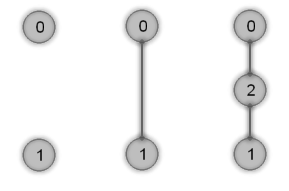
\includegraphics{images/add_att2}
	\caption{Two nodes that share an attribute, how we can link them, 1-no edge, 2-hypergraph, 3-bipartite graph}
	\label{fig:add_att2}
\end{figure}
\begin{figure}[htp]
	\centering
	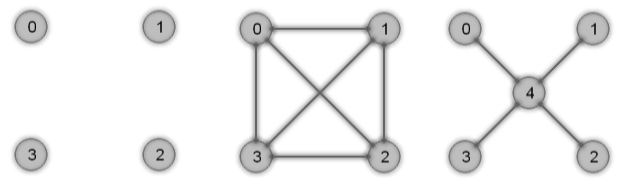
\includegraphics[width=\linewidth]{images/add_att4}
	\caption{Four nodes that share an attribute, how we can link them, 1-no edge, 2-hypergraph, 3-bipartite graph}
	\label{fig:add_att4}
\end{figure}
\\
Then exist two methods to link some nodes through the attribute. In figure~\ref{fig:add_att2} and~\ref{fig:add_att4}, there are two different examples. In both figures we have three scenes, the first one shows the nodes without any linkage, the second one shows the nodes connected directly, in the last one we have the nodes connected across another node that does the hub, this hub is the node taken from the attribute.
Is easy to understand the difference, the second scene, named hypergraph, create a complete graph, this mean that I have  $ \displaystyle\binom{n}{2}$ edges, in figure~\ref{fig:add_att4} are $ \displaystyle\binom{4}{2} = 6$, but no one node is added.\\
The third scene is a star graph that builds a bipartite graph, add a node for each attribute, but only $n$ edges, for figure~\ref{fig:add_att4} this mean that we add one node and four edges.\\
Which one we prefer?\\
It depends on the situations, if there are lots of attributes and each of these is available for a little number of nodes, probably we are going to prefer the hypergraph. If there are some attribute that is available for a high number of nodes probably we prefer the bipartite graph.\\
In fact if for example we have an attribute available for $100$ nodes this mean that with the bipartite graph we add $1$ node and $100$ edges, for the hypergraph we add zero nodes but $ \displaystyle\binom{100}{2} = 4950$ edges.\\
For this reason, we have chosen for use the bipartite graph.\\
To note that when we walk on this new graph we save in the array of walks for both type of nodes, then after walking we must delete the ID of the nodes belonging to the attributes. Because the future steps of the algorithm must not know the existence of the bipartite graph.
%
\subsection{Name of bipartite graph}
I would like to explain where this name does come from. The graph is called bipartite because there are two set of nodes, the nodes that before I called N1 (original nodes) and N2 (nodes from attribute). Every edge of the graph goes from a node of N1 to a node of N2 and vice versa. There is no one edge that goes from N1 to N1 or from N2 to N2. This is perfect for our situation if we had two nodes of N1 linked this would mean that we have not deleted the original edges if we would have two nodes of N2 linked this would mean that we have done an error, two attributes can not be linked.
%
\subsection{Name of hypergraph}
I would like to explain where this name does come from. The hypergraph do not have simple edges but have hyperedges, the normal edges have two endpoints and both are nodes, so its possible to represent it with a line. Differently, the hyperedges do not have two endpoints but potentially an infinite number of endpoints, this allows that a hyperedge link more than two nodes directly. If you want to represent an hyperedges on a normal undirected graph this mean that, if the hyperedges link directly 5 nodes we must replace it with a complete graph on this 5 nodes so we use $ \displaystyle\binom{5}{2} = 10$ normal edges.

Note that, this is exactly our situation, in fact, an attribute link the nodes to which it belongs directly, so we can imagine that for each attribute we are going to create a hyperedge on his nodes.
%
%

\section{Build graph - example}
In this section, I am going to show how a graph is transformed from the simple structure and the attributes to a hypergraph or to a bipartite graph.\\
%
\begin{multicols}{2}
	\begin{center}
		\begin{tabular}{|l|cc|}
		\hline
		ID&\multicolumn{2}{c|}{attributes ID}\\
		\hline
		1&11&\\
		2&11&12\\
		3&10&12\\
		4&11&13\\
		5&11&12\\
		6&12&13\\
		7&13&14\\
		\hline
		\end{tabular}
		\captionof{table}{For each node, there are the attributes ID that it has}
		\label{tab:7_ID_to_att}
		%
		\begin{tabular}{|l|cccc|}
		\hline
		att&\multicolumn{4}{c|}{node ID}\\
		\hline
		10&3&&&\\
		11&1&2&4&5\\
		12&2&3&5&6\\
		13&4&6&7&\\
		14&7&&&\\
		\hline
		\end{tabular}
		\label{tab:7_att_to_ID}
		\captionof{table}{For each attribute, there are the nodes ID that it has}
	\end{center}
\end{multicols}
%
%
\begin{figure}[htp]
	\centering
	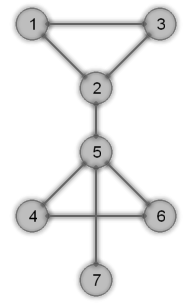
\includegraphics{images/7transform_str}
	\caption{The structure representation of the graph}
	\label{fig:7transform_str}
\end{figure}
%
%
In figure~\ref{fig:7transform_str} we can see the structure of the graph. In table~\ref{tab:7_ID_to_att} we can see that for each node is represented the ID of the attributes that it has. At the opposite in table~\ref{tab:7_att_to_ID} for each attribute, are represented the ID of the nodes that have it.\\
Then now it is possible to create the two graphs.
%
\begin{figure}[htp]
	\centering
	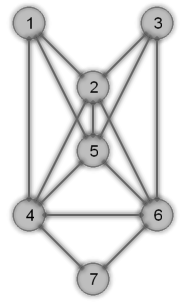
\includegraphics{images/7transform_hyper}
	\caption{The representation of the hypergraph}
	\label{fig:7transform_hyper}
\end{figure}
\\
First, we look at the hypergraph shown in figure~\ref{fig:7transform_hyper}.
\begin{itemize}
	\item  we can see that some edges are no more present, two examples are $(1,3)$ and $(5,7)$, some other before was deleted and after they are replaced
	\item  the nodes that share the same attribute build a complete graph, two example are $[1,2,4,5]$ with the attribute $11$ and $[4,6,7]$ with the attribute $13$
	\item  if only one node has a particular attribute this does not create an edge, this is the case of the two attributes $10$ and $14$
\end{itemize}
%
\begin{figure}[htp]
	\centering
	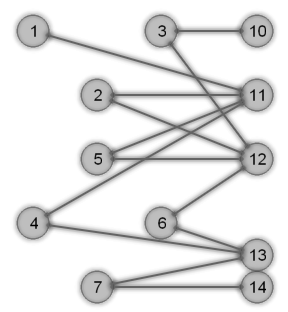
\includegraphics{images/7transform_bipartite}
	\caption{The representation of the bipartite graph}
	\label{fig:7transform_bipartite}
\end{figure}
%
We look now a more complex situation, the bipartite graph shown in figure~\ref{fig:7transform_bipartite}. It is not easy to see what happen.\\
The nodes from 1 to 7, on the left, are the original ones the nodes from 10 to 14 (higher equal than 10), on the right, are the new ones created from the attributes. 
\begin{itemize}
	\item the nodes on the left and the nodes on the right are separate are the two sets of which I spoke before N1 and N2
	\item all edges cross the middle of the graph, go from left to right
	\item all the edges present in the original graph are no more present, we have deleted all of them
	\item the nodes that share the same attribute build a star graph, two example are $[1,2,4,5]$ with the attribute $11$ and $[4,6,7]$ with the attribute $13$
	\item  if only one node has a particular attribute this do not do difference, in fact, the two attributes $10$ and $14$ are anyway linked to the left part
\end{itemize}
%
%
%
%\end{document}
			%capitolo 1
	%%%%%%%%%%%%%%%%%%%%%%%%%%%%%%%%%%%%%%%%%%%%

% formato FRONTE RETRO
\documentclass[epsfig,a4paper,11pt,titlepage,twoside,openany]{book}
\usepackage{epsfig}
\usepackage{plain}
\usepackage{setspace}
\usepackage[paperheight=29.7cm,paperwidth=21cm,outer=1.5cm,inner=2.5cm,top=2cm,bottom=2cm]{geometry} % per definizione layout
\usepackage{titlesec} % per formato custom dei titoli dei capitoli

\singlespacing

\usepackage[italian]{babel}

%%%%%%%%%%%%%%%%% STEFANO ADDED %%%%%%%%%%%%%%%%
% supporto lettere accentate
% queste due righe nel preambolo servono a poter utilizzare le lettere accentate in tutto il testo se no di norma si inserirebbero con \'e...
\usepackage[T1]{fontenc}
\usepackage[utf8]{inputenc}
\usepackage{hyperref} %Serve per i riferimenti
\usepackage{caption}  %Serve per le note (caption)
\usepackage{multicol}	 %Serve per usare più colonne

%%%%%%%%%%%%%%%%% ENRICO ADDED %%%%%%%%%%%%%%%%%
\usepackage{ulem} %Serve per il sottolineato
\usepackage{amsmath} %Serve per alcuni ambienti matematici
\usepackage{array} %Serve per le tabelle
\usepackage{multirow} %Seve per tabelle
\setcounter{secnumdepth}{5} %Utilissimo serve per aumentare il numero di paragrafi, si arriva fino a 5 livelli di profondità x.x.x.x.x
%GRAFICI
\usepackage{pgfplots}
\usepackage{pgfmath}
\usepackage{tikz}
%CODICE
% \usepackage{listings}
% \usepackage[cache=false]{minted} 
%\setminted{tabsize=4, breaklines, breakanywhere, linenos, mathescape,}

% \lstset{
% 	  breakatwhitespace=false,         
% 	  breaklines=true,     
% 	  basicstyle=\footnotesize\ttfamily,            
% 	  commentstyle=\color{blue}, %Indica il colore dei commenti
% 	  keywordstyle=\color{red}, %Indica il colore delle parole chiave
% 	  language=C, %Indica il linguaggio predefinito da usare
% 	  rulecolor=\color{black}, %Indica il colore dei numeri di righe
% 	  tabsize=4,
% 	  escapeinside={\%*}{*)},
% 	  morekeywords={}, %Altre parole da inserire tra le keywords. Ad esempio possiamo aggiungere do, gotttto, ecc ecc 
% }
%%%%%%%%%%%%%%%%% END OF ENRICO  %%%%%%%%%%%%%%%%

\begin{document}
%set the language of the text to italian
% !TeX spellcheck = it_IT

%%%%%%% personal commands (ALIAS):
% \newcommand{\nome_commando}[argomenti]{comando}
\newcommand{\e}[1]{$\cdot 10^{#1}$}
\newcommand{\mmax}[0]{mod\_withMax }
\newcommand{\mover}[0]{mod\_overlap }
\newcommand{\mmod}[0]{modularità modificata }
\newcommand{\nv}[0]{Node2Vec }
\newcommand{\wv}[0]{Word2Vec }
\newcommand{\cnrl}[0]{CNRL }
\newcommand{\cora}[0]{Cora }
\newcommand{\citeseer}[0]{Citeseer }
\newcommand{\LPred}[0]{Link Prediction }
%



%
\chapter{Metodi di valutazione}
Questo capitolo spiega di come si valuta una partizione creata dagli algoritmi d'individuazione delle comunità. Come citato nel sommario, il metodo scelto nel corso del tirocinio è stato la modularità, il cui simbolo è $Q$.\\
La modularità altro non è che un valore solitamente compreso all'interno dell'intervallo $[-1, 1]$. Tuttavia questo non è sempre vero poiché dipende strettamente da quale metodo d'implementazione si va ad utilizzare. Le prime persone che hanno lavorato sulla modularità sono state Newman e Girvan , che necessitavano di un metodo formale per decidere fra due partizioni di nodi quale fosse la migliore.\\
Newman e Girvan  quando hanno scritto le prime applicazioni della modularità sono partiti da una semplice assunzione: un nodo non può appartenere a più di una comunità. Questo elimina tutti i problemi dovuti alla sovrapposizione delle comunità. Per i casi studiati durante il tirocinio quest'assunzione non sempre è valida. Inizialmente è molto comoda poiché permette di ridurre notevolmente la complessità del calcolo della modularità.\\
\\
Durante tutto il lavoro svolto si è passati attraverso tre differenti metodi, tutti e tre verranno ora mostrati ed ove possibile spiegati, si parte dal più semplice fino ad arrivare al più complesso.\\ Durante la spiegazione di ogni metodo viene assunto di lavorare con grafi non orientati, alla fine di ogni sezione sono indicati gli eventuali cambiamenti da applicare in caso si abbia invece a che fare con grafi orientati.
%
\section{Modularità con massimi ( \mmax )}
È stato scelto questo nome in quanto questo metodo gestisce al massimo una comunità per ogni nodo, andando a ricalcare l'assunzione base di Newman e Girvan .\\
L'idea di base è che questo metodo va a calcolare un valore di modularità per ogni comunità. Tutti questi elementi sono poi sommati fra loro per andare a creare il valore di modularità del grafo in se. È necessario far notare che questo metodo non permette la sovrapposizione delle comunità, per l'assunzione fatta, di conseguenza è impossibile che la sommatoria finale vada a considerare più di una volta i valori raccolti, da un qualsiasi elemento del grafo.\\
Questo metodo si basa sull'osservazione che è possibile identificare una comunità sulla base della frequenza degli archi contenuti al suo interno. Di fatto se un insieme di nodi dispone di una grande quantità di archi che li collegano direttamente, questi nodi dovrebbero essere una comunità a sé stante o almeno far parte della stessa. Se così non fosse allora la valutazione della partizione sul grafo deve essere penalizzata in quanto non ha considerato questi nodi come parte dello stesso gruppo.\\
Il motivo per cui è stato scelto questo metodo, oltre al fatto che è semplice da calcolare, è proprio perché va a penalizzare le partizioni che non considerano una comunità molto evidente.\\
Di seguito la formula completa:
\begin{equation}
	Q=\sum_{c}^{C_r} \left( \frac{l_c}{L}-\left(\frac{d_c}{2L} \right)^2 \right)
	\label{eq:m_max}
\end{equation}
Dove gli elementi dell'equazione sono:
\begin{itemize}
	\item $Q$ è il simbolo di modularità
	\item $C_r$ è l'insieme delle comunità calcolate
	\item $c$ è l'iteratore sulle comunità
	\item $L$ è il numero totale di archi all'interno del grafo, solitamente indicato con $m=|E|$
	\item $l_c$ è il numero totale di archi interni alla comunità $c$, questo significa che ognuno degli archi qui contati ha ambo i nodi alle estremità appartenenti alla comunità $c$
	\item $d_c$ è il grado della comunità $c$, definito come la sommatoria dei gradi dei nodi che vi appartengono
\end{itemize}
%
Si può notare che $\frac{l_c}{L}$ è il peso della comunità $c$ rispetto al resto del grafo, in quanto si calcola la percentuale di archi di cui la comunità $c$ dispone. Mentre $\frac{d_c}{2L}$ è la densità di archi tramite cui la comunità $c$ interagisce, ossia quanto, rispetto al totale, sono importanti i nodi che appartengono a questa comunità.\\
\\
Quando si parla di grafo orientato l'unica parte da modificare è $\frac{d_c}{2L}$ che diventa $\frac{d_c}{L}$. In un grafo non orientato un arco incrementa di uno il grado di due nodi, quello  di partenza e quello d'arrivo, mentre, se l'arco fosse orientato questo non accadrebbe in quanto aumenterebbe solamente il grado del nodo di partenza, ecco il motivo del fattore moltiplicativo $2$ di differenza.
%
%
\section{Modularità con sovrapposizione ( \mover )}
L'algoritmo qui descritto è preso dall'articolo intitolato "Modularity measure of networks with overlapping communities"\cite{M-over_paper}.\\
Come si può intuire dal nome questo metodo permette a due comunità di condividere uno o più nodi e quindi d'aver una sovrapposizione. In linea con diversi altri metodi la modularità generata da questo algoritmo cade nell'intervallo $[-1, 1]$.\\
Se nel metodo precedente si calcolava un valore di modularità per ogni comunità e poi li si sommava in quanto non era prevista la sovrapposizione, qui la gestione è simile. Si calcola un valore per ogni comunità e poi, invece di sommarli, se ne ricava una media poiché la sovrapposizione è concessa. Uno stesso nodo può portare il suo contributo a diversi elementi della sommatoria.\\
Di seguito la formula completa:
\begin{equation}
	Q = M^{ov} = \frac{1}{K} 
	\sum_{r=1}^{K} \left[
		\frac
			{\sum\limits_{i \in c_r} 
				\left( \frac
					{
						\sum\limits_{j \in c_r, i \neq j} \left( a_{ij} \right) 
						- 
						\sum\limits_{j \notin c_r} \left( a_{ij} \right) 
					} 
					{d_i \cdot s_i} 
				\right) } 
			{n_{c_r}}
		\cdot
		\frac{ n^e_{c_r} }{ \binom{n_{c_r}}{2} } 
	\right]
	\label{eq:m_over}
\end{equation}
Dove gli elementi dell'equazione sono:
\begin{itemize}
	\item $C_r$ è l'insieme delle comunità calcolate
	\item $K$ è il numero di comunità calcolate, pari a $|C_r|$
	\item $c_r$ è la comunità attuale
	\item $n_{c_r}$ rappresenta il numero di nodi interni alla comunità $c_r$
	\item $n^e_{c_r}$ rappresenta il numero di archi interni alla comunità $c_r$
	\item $\binom{n_{c_r}}{2}$ è il numero massimo di archi potenzialmente presenti nella comunità $c_r$
	\item $d_i$ è il grado del nodo $i$
	\item $s_i$ è il numero di comunità a cui il nodo $i$ appartiene
	\item $a_{ij}$ vale 1 se l'arco dal nodo $i$ al nodo $j$ esiste, altrimenti assume il valore 0
\end{itemize}
%
Ecco spiegati dettagli presenti all'interno di quest'Equazione~\ref{eq:m_over}.\\
Come per il metodo precedente si calcola la densità della comunità (attraverso la Formula~\ref{eq:edge_density}). Ora si confronta il numero di archi interni presenti, rispetto al potenziale numero massimo, ossia il numero di archi presenti in un grafo completo con lo stesso numero di nodi.
\begin{equation}
	\frac{ n^e_{c_r} }{ \binom{n_{c_r}}{2} }
	\label{eq:edge_density}
\end{equation}
%
In aggiunta, si considera la relazione fra il numero di archi interni e quelli uscenti (tramite la Formula~\ref{eq:in-out_edge_relation}). Di conseguenza sembrerebbe che se il numero di archi uscenti è maggiore rispetto al numero di archi interni il valore di modularità vada ad assumere un valore negativo, in caso contrario positivo.\\
\begin{equation}
	\sum\limits_{i \in c_r} \left( \frac{
		\sum\limits_{j \in c_r, i \neq j} \left( a_{ij} \right) - 
		\sum\limits_{j \notin c_r} \left( a_{ij} \right) 
	} {d_i \cdot s_i} \right)
	\label{eq:in-out_edge_relation}
\end{equation}
In realtà non è sempre così, si deve tener conto anche del peso degli elementi $d_i$ e $s_i$. Questi due parametri hanno il compito di assegnare ad ogni arco un valore rappresentativo della sua importanza, interno o uscente è completamente indifferente. Si può notare come il valore di un arco possa variare all'interno dell'intervallo $]0, 1]$. Un arco ha inizialmente valore $1$ e viene poi diviso per due interi positivi moltiplicati fra loro, in seguito viene considerato con peso positivo se favorisce la comunità ossia se è interno, negativo se così non è.\\
$d_i$ è importante perché va a premiare gli archi che partono da un nodo con un basso grado. Il nodo avendo pochi archi, fa si che ognuno di questi sia molto importante, in quanto, la somma totale dei pesi degli archi di un nodo, è un valore costante uguale per tutti i nodi. Inoltre, tramite $s_i$, si premiano i nodi che appartengono a poche comunità, poiché tali nodi meglio rappresentano la loro comunità d'appartenenza. Se un nodo è comune a tutte le comunità del grafo non è per nulla rappresentativo e quindi ogni volta avrà un influenza estremamente bassa.\\
\\
È stato scelto questo metodo poiché permette la sovrapposizione di comunità. Inoltre andando a calcolare un valore di modularità per ogni comunità individuata nel grafo si può facilmente capire quale di queste dà un maggior contributo al risultato finale e quale invece tende solo a penalizzare la partizione a causa della sua bassa coesione.\\
Compresa la formula generatrice, si può notare che un particolare valore di modularità può rivelare  due importanti dettagli del grafo:
\begin{itemize}
	\item un valore negativo sta a significare che i gruppi di nodi non sono densamente connessi al loro interno ma piuttosto legati a punti esterni. Pur con un valore negativo è possibile che gli archi interni siano in numero maggiore rispetto agli archi verso l'esterno, ma, se ciò accade, è perché i parametri di $d_i$ e $s_i$ hanno dato maggior rilevanza agli archi uscenti
	\item se la modularità ha un valore, che in assoluto si avvicina molto allo zero, sta a significare che il grafo valutato è estremamente sparso. Il fattore moltiplicativo mostrato nell'Equazione~\ref{eq:edge_density} va a collassare i vari elementi della formula vicino allo zero, di conseguenza anche la sommatoria non si allontanerà di molto da quel valore
\end{itemize}
Quando si parla di grafo orientato l'unica differenza, da considerare, la si applica alla Formula~\ref{eq:edge_density}. Si dà il caso che il numero massimo di archi in un grafo orientato sia il doppio del numero di archi per lo stesso grafo non orientato, questo per il semplice motivo che si possono creare due archi leganti gli stessi due nodi se presentano versi opposti. Pertanto il numero massimo cambia da $\binom{n_{c_r}}{2}$ per diventare $ 2\binom{n_{c_r}}{2}$.
%
%
\section{Modularità modificata}
Questo algoritmo\cite{M-mod_code} è preso dall'articolo intitolato "Incorporating Implicit Link Preference Into Overlapping Community Detection"\cite{M-mod_paper}.\\
Questo è l'algoritmo che è stato scelto da chi ha scritto l'articolo di \cnrl e, per questa ragione, è stato adottato anche da noi. È estremamente importante perché permette di replicare i risultati illustrati nel documento cui facciamo riferimento. Si ha quindi un punto fisso da cui partire e con cui all'occorrenza confrontarsi.\\
Sfortunatamente questo è il più lento dei tre metodi che vengono illustrati in questo capitolo, per il semplice motivo che è il più complesso, sia logicamente che computazionalmente.\\
Di seguito vi sono due versioni della stessa formula (senza sistema~\ref{eq:m_mod} e con sistema~\ref{eq:m_mod_system}):
\begin{equation}
	Q = \frac{1}{M} \cdot \sum_{u,v \in V}
		\left[
			\left( A \left[ u,v \right] - \frac{ d_{in}\left(u\right) \cdot d_{out}\left(v\right) }{M} \right)
			\cdot
			|C_u \cap C_v| 
		\right]
	\label{eq:m_mod}
\end{equation}
%
\begin{equation}
	Q = \frac{1}{M} \cdot \sum_{u,v \in V}
		\begin{cases}
			\begin{array}{ll}
				0 & |C_u \cap C_v| = 0 \\
				\left[ \left( A \left[ u,v \right] - \frac{ d_{in}\left(u\right) \cdot d_{out}\left(v\right) }{M} \right) \cdot |C_u \cap C_v| \right]
				& altrimenti
			\end{array}
		\end{cases}
	\label{eq:m_mod_system}
\end{equation}
Dove gli elementi delle equazioni sono:
\begin{itemize}
	\item $M$ può assumere due valori a seconda che il grafo sia orientato o no, ossia misura $m$ se indiretto assume invece il valore $2m$ se diretto.\\
	In tutto questo $m$ è il numero di archi del grafo, ossia come di norma $m=|E|$
	\item $u,v$ sono gli iteratori sui nodi del grafo, chiamati come di consueto $V$
	\item $A \left[ u,v \right]$ rappresenta il peso assunto dall'arco $(u, v)$. Se tale arco non esiste il valore è $0$, mentre se l'arco esiste il peso è un valore positivo, di default $1$
	\item $d_{in}\left(u\right)$ e $d_{out}\left(u\right)$ sono i gradi entranti e uscenti del nodo $u$, questi rispettivamente contano il numero di archi entranti e uscenti dal nodo.\\
	Se il grafo è indiretto, questi due valori, preso un qualsiasi nodo, saranno perfettamente uguali
	\item $C_u$ è l'insieme delle comunità a cui il nodo $u$ appartiene
	\item $|C_u \cap C_v|$ è il numero totale di comunità condivise fra i nodi $u$ e $v$
\end{itemize}
%
Come per i metodi precedenti segue una spiegazione delle varie sezioni di tale Formula~\ref{eq:m_mod}.\\
Si prende l'elemento $ |C_u \cap C_v|$: questo fattore moltiplicativo ci permette d'ignorare gli archi che legano nodi che non condividono nessuna comunità. Per capire il suo scopo si può pensare ad una partizione che non presenta sovrapposizioni, in questo caso tale componente permetterà di ignorare tutti gli archi che non sono interni ad una singola comunità, ma passano da una all'altra. Ignorando ora l'assunzione base di Newman e Girvan  si può dire che gli unici archi considerati sono quelli che rimangono interni ad almeno una comunità, anche se è permesso loro essere di collegamento fra altre. Il funzionamento di questo componente è illustrato bene nella seconda versione (Formula~\ref{eq:m_mod_system}), grazie al sistema si nota che se la condizione è verificata si può ignorare tutta la prima parte.\\
Oltre a filtrare gli archi utilizzabili questo componente assegna un importanza maggiore a quegli archi che connettono nodi che condividono molte comunità.
\begin{equation}
	\frac{ d_{in}\left(u\right) \cdot d_{out}\left(v\right) }{M}
	\label{eq:d_in-out}
\end{equation}
La base che si ignora o moltiplica è un valore positivo, se l'arco esiste (questo grazie ad $ A \left[ u,v \right]$), mentre assume un valore negativo se l'arco non c'è, in quanto al peso $0$ dell'arco inesistente si sottrae il fattore definito nella Formula~\ref{eq:d_in-out}.\\
Quest'espressione rappresenta la rilevanza di un arco, indipendentemente dalla sua esistenza. Se tale arco collega due nodi con gradi elevati risulta essere uno fra molti e quindi ha un'importanza limitata, se diversamente collega nodi con gradi bassi allora assume molta più importanza perché è un caso isolato e quindi prezioso.
%\end{document}



	%capitolo 2
    %%%%%%%%%%%%%%%%%%%%%%%%%%%%%%%%%%%%%%%%%%%%

% formato FRONTE RETRO
\documentclass[epsfig,a4paper,11pt,titlepage,twoside,openany]{book}
\usepackage{epsfig}
\usepackage{plain}
\usepackage{setspace}
\usepackage[paperheight=29.7cm,paperwidth=21cm,outer=1.5cm,inner=2.5cm,top=2cm,bottom=2cm]{geometry} % per definizione layout
\usepackage{titlesec} % per formato custom dei titoli dei capitoli

\singlespacing

\usepackage[italian]{babel}

%%%%%%%%%%%%%%%%% STEFANO ADDED %%%%%%%%%%%%%%%%
% supporto lettere accentate
% queste due righe nel preambolo servono a poter utilizzare le lettere accentate in tutto il testo se no di norma si inserirebbero con \'e...
\usepackage[T1]{fontenc}
\usepackage[utf8]{inputenc}
\usepackage{hyperref} %Serve per i riferimenti
\usepackage{caption}  %Serve per le note (caption)
\usepackage{multicol}	 %Serve per usare più colonne

%%%%%%%%%%%%%%%%% ENRICO ADDED %%%%%%%%%%%%%%%%%
\usepackage{ulem} %Serve per il sottolineato
\usepackage{amsmath} %Serve per alcuni ambienti matematici
\usepackage{array} %Serve per le tabelle
\usepackage{multirow} %Seve per tabelle
\setcounter{secnumdepth}{5} %Utilissimo serve per aumentare il numero di paragrafi, si arriva fino a 5 livelli di profondità x.x.x.x.x
%GRAFICI
\usepackage{pgfplots}
\usepackage{pgfmath}
\usepackage{tikz}
%CODICE
% \usepackage{listings}
% \usepackage[cache=false]{minted} 
%\setminted{tabsize=4, breaklines, breakanywhere, linenos, mathescape,}

% \lstset{
% 	  breakatwhitespace=false,         
% 	  breaklines=true,     
% 	  basicstyle=\footnotesize\ttfamily,            
% 	  commentstyle=\color{blue}, %Indica il colore dei commenti
% 	  keywordstyle=\color{red}, %Indica il colore delle parole chiave
% 	  language=C, %Indica il linguaggio predefinito da usare
% 	  rulecolor=\color{black}, %Indica il colore dei numeri di righe
% 	  tabsize=4,
% 	  escapeinside={\%*}{*)},
% 	  morekeywords={}, %Altre parole da inserire tra le keywords. Ad esempio possiamo aggiungere do, gotttto, ecc ecc 
% }
%%%%%%%%%%%%%%%%% END OF ENRICO  %%%%%%%%%%%%%%%%

\begin{document}
%set the language of the text to italian
% !TeX spellcheck = it_IT

%%%%%%% personal commands (ALIAS):
% \newcommand{\nome_commando}[argomenti]{comando}
\newcommand{\e}[1]{$\cdot 10^{#1}$}
\newcommand{\mmax}[0]{mod\_withMax }
\newcommand{\mover}[0]{mod\_overlap }
\newcommand{\mmod}[0]{modularità modificata }
\newcommand{\nv}[0]{Node2Vec }
\newcommand{\wv}[0]{Word2Vec }
\newcommand{\cnrl}[0]{CNRL }
\newcommand{\cora}[0]{Cora }
\newcommand{\citeseer}[0]{Citeseer }
\newcommand{\LPred}[0]{Link Prediction }
%



%
\chapter{Esperimenti}
\section{Origini dei grafi}
In questa sezione vengono spiegati i dataset utilizzati e cosa rappresentano.\\
Si possono dividere in due gruppi, in quanto presentano caratteristiche d'affinità, ma anche perché i grafi dei due gruppi sono stati utilizzati nel corso del tirocinio per tre applicazioni differenti.\\
Nella Tabella~\ref{tab:dati_grafi} sono elencati i dettagli tecnici di ogni dataset.
%
\begin{center}
	\begin{tabular}{|l|r|r|r|c|c|r|}
		\hline
		nome&nodi&archi&archi/nodi&diretto&etichette&attributi\\
		\hline
		\cora & 2708 & 5429 & 2.0 & sì & 7 & 1433\\
		\citeseer & 3312 & 4732 & 1.4 & sì & 6 & 3703\\
		\hline
		BlogCatalog & 10312 & 333983 & 32.4 & no & 39 & 0\\
		Gnutella & 6301 & 20777 & 3.3 & no & 0 & 0\\
		Dolphins & 62 & 159 & 2.6 & no & 0 & 0\\
		Karate & 35 & 78 & 2.2 & no & 0 & 0\\
		\hline
		\end{tabular}
		\captionof{table}{Per ogni grafo sono indicate le sue caratteristiche principali}
		\label{tab:dati_grafi}
\end{center}
%
\subsection*{Esperimento principale: \cora - \citeseer}\cite{Co-Ci_1}\cite{Co-Ci_2}
Il dataset di \textbf{\cora} è un grafo diretto che rappresenta una rete di articoli scientifici sull'apprendimento automatico, ogni nodo è un articolo. Mentre ogni arco rappresenta il collegamento fra un documento è l'altro, se il documento $A$ cita il documento $B$ si avrà l'arco $(A, B)$. La rete è costruita in modo che ogni nodo abbia almeno un arco entrante o uscente.\\
Ogni articolo appartiene ad esattamente una classe identificata da un etichetta. Ogni attributo rappresenta la presenza (deve apparire almeno 10 volte) o meno di una determinata parola nel testo del documento.\\
\\
Il dataset di \textbf{\citeseer} è un grafo diretto che rappresenta una rete analoga a quella di \cora, anche qui si hanno articoli scientifici che si citano vicendevolmente. L'etichetta è la classe d'appartenenza di cui l'articolo fa parte, e gli attributi son nuovamente la presenza o meno di certe parole all'interno del testo.\\
%
\subsection*{Grafi per esperimenti minori}
Questi quattro grafi vengono presentati in ordine decrescente nel numero dei nodi, così come fatto nella seconda parte della Tabella~\ref{tab:dati_grafi}.\\
\begin{itemize}
	\item \textbf{BlogCatalog}\cite{BlogCatalog} rappresenta la rete di relazioni, di conoscenza, fra gli utenti di alcune piattaforme per blog
	\item \textbf{Gnutella}\cite{Gnutella_1}\cite{Gnutella_2} questo grafo si rifà alla rete peer-to-peer per lo scambio di file di Gnutella nell'agosto 2002. Ogni nodo rappresenta un host e ogni arco un collegamento fra due host
	\item \textbf{Soc-Dolphins}\cite{Dolphins_1}\cite{Dolphins_2} riporta la rete sociale di un gruppo di delfini al largo della Nuova Zelanda nel 2003
	\item \textbf{Karate}\cite{Karate} raccoglie lo storico degli incontri in un club di karate universitario nel 1977. Ogni nodo è un membro del club, ogni arco indica uno scontro terminato in pareggio
\end{itemize}
%
\section{Modello di un grafo}
In questa sezione viene spiegato cosa si intende per modello di un grafo, e perché è tanto importante per gli algoritmi che vi sono costruiti sopra.\\
Come descritto nel capitolo sull'implementazione è necessario visitare il grafo per generare su questo dei cammini. Tali vettori di nodi vengono presi in input dall'algoritmo di \wv che tramite una rete neurale va a descrivere ogni nodo che coinvolto tramite un vettore di valori reali, mentre \cnrl utilizza un metodo alternativo chiamato Latent Dirichlet Allocation (LDA)\cite{LDA} o in alternativa una sua variante detta HalfLDA, entrambe sono comunque basate su \wv.\\
\begin{figure}[htp]
	\centering
	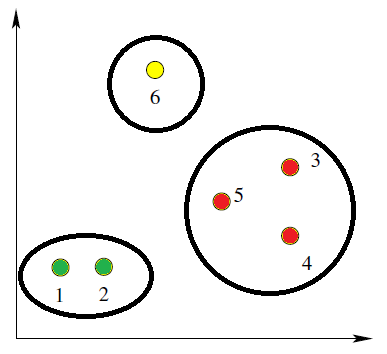
\includegraphics{immagini/punti_modello}
	\caption{Son visualizzati i nodi d'un grafo che vengono rappresentati da un modello che dispone di due dimensioni, mostrato in Tabella~\ref{tab:coordinate_modello}}
	\label{fig:grafico_modello}
\end{figure}
\\
\begin{center}
	\begin{tabular}{|l|cc|}
		\hline
		ID&X1&X2\\
		\hline
		1 & 1 & 2\\
		2 & 2 & 2\\
		3 & 7 & 5\\
		4 & 7 & 3\\
		5 & 5 & 4\\
		6 & 3 & 8\\
		\hline
	\end{tabular}
	\captionof{table}{Tabella rappresentativa del modello dei nodi in Figura~\ref{fig:grafico_modello}}
	\label{tab:coordinate_modello}
\end{center}
Di norma ogni vettore è lungo $64$, e ogni numero reale rappresenta una posizione lungo un asse in uno spazio a $64$ dimensioni. È possibile pensare anche ad un caso più semplice, ad esempio in Figura~\ref{fig:grafico_modello} si possono vedere sei punti che si può immaginare appartenessero ad un grafo e fossero legati fra loro in qualche modo. Una volta che son stati generati i cammini su tale grafo, e questi forniti ad uno dei due algoritmi, viene ritornata la Tabella~\ref{tab:coordinate_modello} dove ad ogni ID di un nodo vengono associati due valori (qui interi per semplicità), vengono ora usati due valori perché son facili da mostrare con $64$ sarebbe pressoché impossibile. Si possono dunque immaginare come coordinate su un piano cartesiano, ed è così che si arriva alla Figura~\ref{fig:grafico_modello}, visivamente si può dire che esistono 3 gruppi distinti evidenziati dai colori, abbiamo quindi $(1, 2) - (3, 4, 5) - (6)$.\\
Escludendo l'influenza causata dai colori, il nostro occhio ci suggerisce l'esistenza di questi 3 gruppi in quanto i nodi che vi fanno parte sono vicini fra loro, questo ricalca alla perfezione la definizione di somiglianza, tanto più due nodi sono vicini tanto più questi sono simili. Si ricorda che esistono comunque molte definizioni formali di somiglianza e la distanza euclidea è solo una di queste.\\
\\
Se due nodi molto simili, e quindi vicini, vengono collegati da un arco allora tale arco assume un valore molto elevato, vicino a $1$, diversamente assumerà un valore molto basso, vicino a $0$, se i nodi che lega sono diversi ossia molto lontani.\\
Questo valore verrà chiamato d'ora in avanti coerenza di un arco\footnote{Non esiste un vero e proprio termine tecnico per questa definizione}.
%
\section{Link Prediction}
Questo è il primo di tre algoritmi, che verranno spiegati in questo capitolo, tutti e tre basati sul modello del grafo appena spiegato.\\
L'algoritmo di \LPred ha lo scopo d'assegnare un valore al grafo in input, questo valore è una percentuale e per tale motivo ricade nell'intervallo $[0, 1]$. Questa percentuale sta a rappresentare la coerenza degli archi del grafo, nel dettaglio un arco è molto coerente se lega due nodi simili, un grafo è tanto più coerente tanti più archi coerenti ha.
%
\subsection{Dinamiche di funzionamento}
In prima istanza viene caricato il grafo, sempre come lista d'archi in quanto sono questi il fulcro dell'algoritmo. Si va poi a spezzare gli archi in due gruppi, dopo averli mescolati per non creare delle divisioni sempre uguali, tale separazione viene fatta sulla base del parametro $F$ che indica quale sarà la percentuale degli archi adibiti all'addestramento del modello e quali invece saranno adibiti alla fase di test.\\
Il numero degli archi usati per il test viene dato dalla Formula~\ref{eq:n_archi_fake}
\begin{equation}
	m \cdot \frac{1}{F}
	\label{eq:n_archi_fake}
\end{equation} 
\begin{equation}
	m \cdot \left( 1- \frac{1}{F} \right)
	\label{eq:n_archi_true}
\end{equation}
mentre quelli utilizzati per l'addestramento corrispondono alla Formula~\ref{eq:n_archi_true}, dove $m$ è il numero di archi del grafo.\\
Il nuovo grafo (\textbf{G1}) creatosi, inseguito alla rimozione degli archi per il test, viene utilizzato per generare il modello.\\
Per ogni arco appartenente all'insieme di test (\textbf{Test=T}) se ne genera un altro (\textbf{Check=C}) tramite una coppia di nodi casuali assicurandosi che non corrispondano ad un arco già esistente. Si hanno quindi tre insiemi, il primo adibito all'addestramento stabilisce il modello necessario a discernere, quale delle due restanti selezioni, è la migliore.
Per ogni arco, di T e di C, si va a veder quanto sono simili i nodi che lega e se ne calcola così la coerenza, grazie all'apposita funzione di similarità, ora disponibile. Gli archi possono essere valutati sulla base di questo nuovo parametro.\\
Si è interessati a capire quanto sono buoni gli archi originari del grafo, T, rispetto a quelli generati casualmente, C. 
\begin{equation}
	\frac{\left( n_1 + \frac{n_2}{2} \right)}{n}
	\label{eq:AUC_formula}
\end{equation}
Si usa perciò la metrica detta AUC\cite{AUC_metric}, che si basa sulla Formula~\ref{eq:AUC_formula}, i cui elementi sono:
\begin{itemize}
	\item $n$ è il numero di archi presenti nell'insieme di test, calcolato mediante la Formula~\ref{eq:n_archi_fake}
	\item $n1$ sono le volte in cui un arco di test T è migliore di un arco casuale di C
	\item $n2$ sono le volte in cui un arco di test T ha pari valore o quasi rispetto ad un arco casuale di C
\end{itemize}
Per ogni arco di T se ne associa casualmente un altro di C, e si guarda quanto valgono i due archi coinvolti se l'arco di T vale più dell'arco di C si incrementa di $1$ il valore di AUC se uguali o quasi (differenza inferiore ad una soglia detta $\displaystyle \epsilon$) si incrementa di $0.5$. Avendo fatto ciò con ogni arco se ne calcola la media.\\
\\
Il valore finale della metrica AUC dipende fortemente da quale metodo si adotta per abbinare gli archi appartenenti a T e C, un accoppiamento sbagliato può fortemente sbilanciare il risultato, è per questo motivo che si va ad utilizzare un abbinamento casuale.\\
Il parametro $F$ influisce sul risultato finale, infatti più questo si avvicina a $1$ più cresce il numero di archi da utilizzare per la selezione di test, diminuiscono di conseguenza i dati su cui fare affidamento per creare un buon modello che rappresenti appieno il grafo di partenza, quindi il valore finale da aspettarsi è tendenzialmente più basso.\\
È necessario ricordare che la stima qui calcolata dipende fortemente dalla selezione iniziale, ed è per questo motivo che tutto questo processo non viene svolto solo una volta bensì $F$ volte, così da andare a stabilizzare il valore calcolato tramite la media di tutte le iterazioni. Inoltre questo permette di utilizzare via via tutti gli archi per addestrare il modello di \textbf{G1}.\\
\\
L'intero algoritmo si basa su confrontare gli archi grazie al valore che li rappresenta per individuare i più rilevanti, quindi la parte critica e più importante è la generazione di tale valore mediante la funzione di similarità.\\
Questa può essere definita in svariate maniere differenti in quanto si possono pesare diversi aspetti. Un esempio classico è basato sulla distanza euclidea più due nodi sono distanti nella rappresentazione del modello meno sono simili. Verranno mostrate le applicazioni di altre funzioni di similarità basate su diversi principi che però non verranno qui riportati.
%
\subsection{Esempio}
\begin{center}
	\begin{tabular}{|c|c|c|c|}
		\hline
		arco & autentico & dist & AUC\\
		\hline
		3-4 & sì & $2$ & \multirow{2}{*}{$1$}\\
		2-6 & no & $\sqrt{37}$ & \\
		\hline
		4-5 & sì & $\sqrt{5}$ & \multirow{2}{*}{$0.5$}\\
		3-5 & no & $\sqrt{5}$ & \\
		\hline
		5-6 & sì & $\sqrt{20}$ & \multirow{2}{*}{$0$}\\
		2-5 & no & $\sqrt{13}$ & \\
		\hline
		1-2 & sì & $1$ & \multirow{2}{*}{$1$}\\
		1-3 & no & $\sqrt{45}$ & \\
		\hline
	\end{tabular}
	\captionof{table}{Tabella riassuntiva del procedimento di \LPred}
	\label{tab:dati_es_prediction}
\end{center}
Si consideri il modello descritto tramite la Figura~\ref{fig:grafico_modello} e la Tabella~\ref{tab:coordinate_modello}. Si sa inoltre che $F=2$, gli archi originali adibiti al test sono $(1, 2), (3, 4), (4, 5), (5, 6)$ mentre quelli generati casualmente sono $(3, 5), (2, 5), (2, 6), (1, 3)$, i due insiemi sono nello stesso numero per creazione e perché così possono essere facilmente confrontati.\\
Nelle prime due colonne della Tabella~\ref{tab:dati_es_prediction} sono riassunti gli archi e la loro origine. Le colonne seguenti rappresentano invece i passaggi successivi dell'algoritmo.\\
Nella terza colonna si può notare che ad ogni arco è stato associato un valore che rappresenta la distanza euclidea misurata sul piano cartesiano generato dal modello fra i due estremi dell'arco. La funzione di similarità premia i valori più bassi a discapito degli altri. Inoltre la Tabella è stata ordinata in modo che tutti gli archi di un insieme siano associati con uno dell'altro in maniera casuale, si può notare  infatti che nella seconda colonna "sì" e "no" s'alternano.\\
Nell'ultima colonna viene rappresentato l'incremento che si andrà ad apportare alla metrica AUC grazie alla valutazione dei due archi corrispondenti. Questo valore dovrà poi esser diviso per il numero delle coppie in gioco per riportarlo nell'intervallo $[0, 1]$, in questo caso risulta $\displaystyle \frac{\left( 1+0.5+0+1 \right)}{4} = 0.625$\\
Si possono osservare alcune peculiarità:
\begin{itemize}
	\item l'accoppiamento degli archi viene fatto in maniera casuale per evitare uno sbilanciamento
	\item nel caso mostrato una selezione a favore degli archi autentici porterebbe ad avere un incremento nullo del valore di AUC, al contrario si potrebbe avere un incremento di due unità se si favorissero  gli archi generati casualmente
	\item non si hanno archi ripetuti perché viene impedito alla creazione, ma questo non vuol dire che un arco di C non possa corrispondere ad un arco usato in principio per generare il modello
	\item si può immaginare che più il valore di $F$ è grande e quindi più è grande la selezione di archi per l'addestramento (grazie alla Formula~\ref{eq:n_archi_true}), più il valore di AUC calcolato cresca
\end{itemize}
L'algoritmo prevederebbe una seconda iterazione di tutto questo procedimento utilizzando gli archi in principio scartati come nuova base per il modello per poi calcolare la media delle percentuali.\\
Si omette questa fase perché uguale a quella appena illustrata.
%
\subsection{Applicazioni}
Le similarità utilizzate in questi esempi sono\cite{all_metric}:
\begin{itemize}
	\item DW = DeepWalk
	\item CN = Common Neighbors\cite{CN_metric}
	\item Salton = Salton Index\cite{Salton_metric}
	\item Jaccard = Jaccard Index
	\item RA = Resource Allocation\cite{RA_metric}
\end{itemize}
%
\begin{figure}[htp]
	\centering
	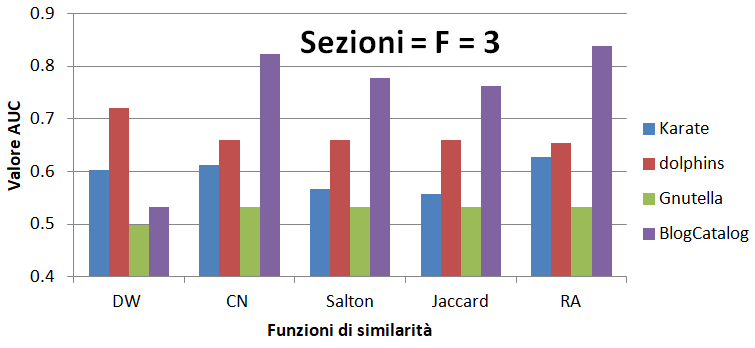
\includegraphics[width=\linewidth]{immagini/LP_fold3}
	\caption{\LPred con tre sezioni, $F=3$}
	\label{fig:LP_fold3}
\end{figure}
%
\begin{figure}[htp]
	\centering
	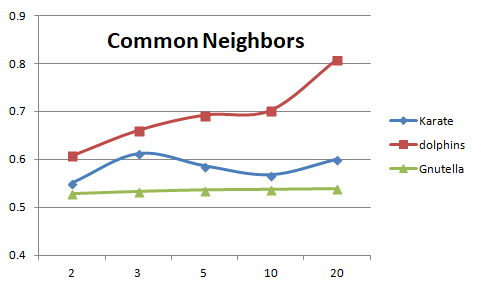
\includegraphics[width=\linewidth]{immagini/LP_CN}
	\caption{Andamento della metrica di Common Neighbors, su tre grafi distinti attraverso differenti percentuali di selezione}
	\label{fig:LP_CN}
\end{figure}
%
\begin{figure}[htp]
	\centering
	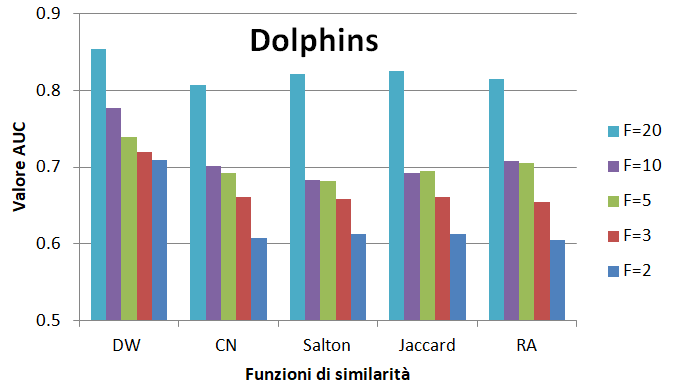
\includegraphics[width=\linewidth]{immagini/LP_Dolphins}
	\caption{Andamento del grafo dolphins su diverse metriche attraverso differenti percentuali di selezione}
	\label{fig:LP_Dolphins}
\end{figure}
%
Questo algoritmo ha tre possibili variabili su cui si può lavorare:
\begin{itemize}
	\item \textbf{Il parametro $F$} (dall'inglese fold) viene fissato nella Figura~\ref{fig:LP_fold3}, si può notare come ogni grafo abbia un livello su cui si attesta, BlogCatalog grazie al fatto che è estremamente denso ha un valore in media molto alto rispetto ai tre grafi restanti
	\item Nella Figura~\ref{fig:LP_CN} si lavora su un \textbf{unica metrica}, si utilizza solo la funzione di similarità denominata Common Neighbors, che si basa sui nodi geometricamente vicini agli estremi di un arco all'interno del modello del grafo per valutare la somiglianza.\\
	Si può notare come all'aumentare del parametro $F$ il valore che si associa ad ogni grafo tende ad aumentare, questo è dovuto ad un modello meglio addestrato perché dispone di più dati in partenza, e quindi si ha una migliore valutazione
	\item La Figura~\ref{fig:LP_Dolphins} è forse la più semplice da osservare in quanto si osserva \textbf{un solo grafo}. Come prima si vede che l'influenza del parametro $F$ sul risultato finale è altissima, inoltre si può notare che le prestazioni di DeepWalk sono leggermente più alte rispetto al resto che invece tende ad avere le stesse performance 
\end{itemize}
Si precisa che questi sono degli esempi rappresentativi dell'andamento generale, che però non viene riportato in quanto sarebbe molto complesso da comprendere.
%
\section{Classificazione dei nodi}
Il problema della classificazione dei nodi/vertici punta a riconoscere partendo dalla rappresentazione di un elemento a quale classe questo appartenga, per definizione un elemento può appartenere ad una ed una sola classe, è tuttavia possibile pensare a classi interne ad altre classi o a sovrapposizioni. Per esempio data la classe A e la classe B si ha che, per come sono state definite, tutti gli elementi di A appartengono anche a B ($\displaystyle A \subseteq B$) di conseguenza $\displaystyle A \cap B = A$, tuttavia questo vale per l'insiemistica, nei problemi di classificazione fra A e B non c'è nessuna relazione e conseguentemente si ha che $\displaystyle A \cap B = \emptyset$.%esempio anche per intersezione???
%
\subsection{Dinamiche di funzionamento}
Il punto di partenza è costante, dato il grafo lo si visita per generare i cammini e con questi s'invoca l'algoritmo che genera il modello. Il modello viene disordinato e spezzato secondo il parametro di training ratio $T_r$, ossia la percentuale d'addestramento, questo indica la percentuale del modello che dovrà essere usata per l'addestramento, la restante sarà per i test.\\
In aggiunta si considerano anche le etichette o classi d'appartenenza, quindi per ogni nodo si ha una tripletta contenente:
\begin{itemize}
	\item ID del nodo che può anche essere dimenticato
	\item il vettore di numeri reali che lo rappresenta, vengono presi dal modello
	\item l'identificativo della classe a cui si appartiene
\end{itemize}
Con questi dati viene addestrata la \textbf{funzione di classificazione}, o \textbf{classificatore}, il cui scopo sarà predire la classe d'appartenenza dato in input il vettore di un qualsiasi nodo.\\
\\
In seguito per ogni nodo appartenente all'insieme di test si cerca di predire la sua classe sottoponendo il suo vettore al classificatore e una volta terminato si confronta se l'esito corrisponde con la reale classe, nota grazie allo stesso file di etichette utilizzato per l'addestramento.\\
È importante far notare che il modello viene spezzato in due perché il classificatore deve essere addestrato su dati diversi da quelli che prenderà in seguito in input, altrimenti non ci sarebbe nulla da predire in quanto i dati passati vengono ricordati e quindi è impossibile sbagliare a dare una risposta.\\
\\
La valutazione delle predizioni effettuate può avvenire mediante un metodo semplice ossia il \textbf{tasso d'errore}, che corrisponde alla Formula~\ref{eq:tasso_errore}, si contano quanti errori si son fatti rispetto al totale o si usa il metodo opposto ossia \textbf{l'accuratezza}, definita nella Formula~\ref{eq:accuratezza}, che conta i risultati con esito positivo rispetto al totale.
%
\begin{equation}
	T_{err} = \frac{N(errori)}{N(previsioni)}
	\label{eq:tasso_errore}
\end{equation}
%
\begin{equation}
	Acc = 1 - T_{err} = 1 - \left( \frac{N(errori)}{N(previsioni)} \right) = \frac{N(corretti)}{N(previsioni)}
	\label{eq:accuratezza}
\end{equation}
%
Se si vogliono fare delle misurazioni particolari si sfrutta invece la \textbf{matrice di confusione}, mostrata in Tabella~\ref{tab:matrice_confusione}, ideata inizialmente per valutare casi con solo due opzioni (Sì-positivo / No-negativo), può essere generalizzata per gestire la valutazione di un classificatore con più di due esiti, tramite due metodi differenti.
\begin{itemize}
	\item si amplia la matrice per avere invece che due righe e due colonne, K righe e colonne.\\
	Dove K è il numero di possibili valori ritornati dal classificatore
	\item si possono creare K matrici di confusione e ogni volta si sceglie una specifica classe come positiva tutte le altre vengono implose nel valore negativo
\end{itemize}
%
\begin{multicols}{2}
\begin{center}
	\begin{tabular}{cc|c|c|}
		 &  & \multicolumn{2}{|c|}{Previsione}\\
		 &  & Sì & No\\
		 \hline
		 Risposta & Sì & TP & FN\\
		 \hline
		 corretta & No & FP & TN\\
		\hline
	\end{tabular}
	\captionof{table}{Viene rappresentata una matrice di confusione}
	\label{tab:matrice_confusione}
	%
	\begin{tabular}{|c|c|}
		\hline
		TP & True Positive \\
		FN & False Negative \\
		FP & False Positive \\
		TN & True Negative \\
		\hline
	\end{tabular}
	\label{tab:MC_significato}
	\captionof{table}{Significato delle sigle della matrice di confusione}
\end{center}
\end{multicols}
%
Da questa matrice possiamo estrarre diverse misurazioni:
\begin{itemize}
	\item \textbf{accuratezza} qui prende una nuova formulazione: $\displaystyle Acc = \frac{TP + TN}{TP + TN + FP + FN} $
	\item \textbf{sensibilità} penalizza le risposte negative sbagliate di conseguenza è meglio dare per positivo un esito se non è certo.\\
	Definita come: $\displaystyle S = \frac{TP}{TP + FN} $
	\item \textbf{precisione} penalizza le risposte positive sbagliate di conseguenza è meglio dare per negativo un esito se non è certo.\\
	Definita come: $\displaystyle P = \frac{TP}{TP + FP} $
	\item \textbf{Macro} precisione/sensibilità è la media aritmetica fra più valori di S o di P.\\
	Definita come: $\displaystyle Macro_{S} = \frac{S_1 + ... + S_n}{n} $
	\item \textbf{Micro} precisione/sensibilità è la media aritmetica delle componenti di S o di P prima di calcolarle, per poi considerarle un unica S o P.\\
	Definita come: $\displaystyle Micro_{P} = \frac{TP_1 + ... + TP_n }{ (TP_1 + ... + TP_n) + (FP_1 + ... + FP_n) } $
	\item \textbf{F1-Score} è la media armonica di: micro/macro/normale sensibilità e precisione.\\
	Definita come: $\displaystyle F1-Score = \frac{2}{ \frac{1}{S} + \frac{1}{P} } = \frac{2 \cdot S \cdot P}{ S + P }$
\end{itemize}
Nel caso mostrato sensibilità e precisione non possono essere utilizzate in quanto ci sono troppi dati, mentre usare micro e macro non ha senso in quanto le classi sono perfettamente equivalenti, di conseguenza premiarne una a discapito di un'altra non ha significato. Per questo se serve si adotta l'F1-score. Tuttavia questa procedura non è veloce da calcolare pertanto spesso si adotta il più semplice e veloce metodo dell'accuratezza.
%
\subsection{Esempio}
\begin{center}
	\begin{tabular}{|c|c|c|c|c|}
		\hline
		ID & x & Previsione & Classe & Corretta\\
		\hline
		$5$ & $9$ & $0$ & $1$ & $0$\\
		$1$ & $13$ & $0$ & $0$ & $1$\\
		$2$ & $15$ & $0$ & $0$ & $1$\\
		$3$ & $27$ & $0$ & $1$ & $0$\\
		$4$ & $34$ & $1$ & $1$ & $1$\\
		$8$ & $36$ & $1$ & $0$ & $0$\\
		$6$ & $48$ & $2$ & $2$ & $1$\\
		$7$ & $59$ & $2$ & $2$ & $1$\\
		\hline
	\end{tabular}
	\captionof{table}{Tabella riassuntiva del procedimento di classificazione dei vertici}
	\label{tab:dati_es_classify}
\end{center}
Tutti i dati dell'esempio sull'algoritmo di classificazione sono riassunti nella Tabella~\ref{tab:dati_es_classify}. Nella prima colonna abbiamo gli ID dei nodi coinvolti, elemento che l'algoritmo ignora completamente. La seconda colonna contiene il vettore rappresentativo di ogni nodo, qui per semplicità è stato ridotto ad un solo numero.
%
\begin{equation}
	C(x)=
		\begin{cases}
			\begin{array}{ll}
				0 & se \ x < 30\\
				1 & se \ 30 \leq x \ \&\  x < 45\\
				2 & se \ 45 \leq x
			\end{array}
		\end{cases}
	\label{eq:classificatore_esempio}
\end{equation}
%
Si assume il classificatore definito nella Formula~\ref{eq:classificatore_esempio}, che darà come risposte i valori contenuti nella colonna "Previsione".\\
Mentre nella colonna "Classe" mostra il valore autentico del nodo. Infine nell'ultima colonna è indicato se la previsione è risultata corretta o meno.\\
\\
Per una valutazione mediante accuratezza è sufficiente calcolare la media aritmetica dell'ultima colonna, ossia $\displaystyle Acc = \frac{1+1+1+1+1}{8} = \frac{5}{8} = 0.625$. Mentre per l'F1-score sarebbe necessario calcolare sensibilità e precisione di ognuna delle 3 classi, riassumerli mediante micro o macro, ed infine arrivare ad un valore con F1-score.
%
\subsection{Applicazioni}
I grafi scelti per questa applicazione sono \cora (Figura~\ref{fig:VC_cora}) e \citeseer (Figura~\ref{fig:VC_citeseer}) perché fra quelli presentati nella Tabella~\ref{tab:dati_grafi} sono gli unici che sono forniti di attributi sui nodi, e questo permette di mostrare come l'utilizzo del grafo bipartito per l'introduzione degli attributi modifica le prestazioni.
%
\begin{figure}[htp]
	\centering
	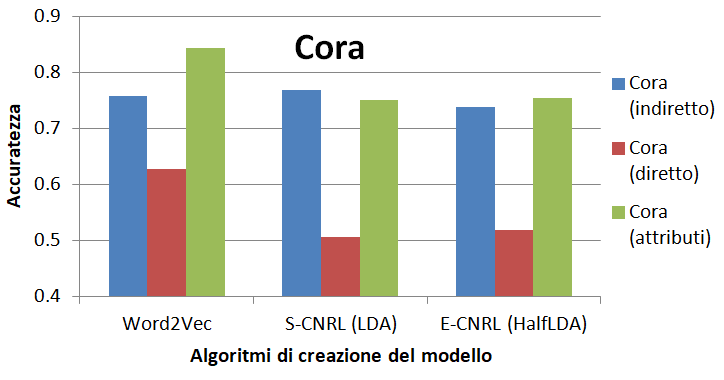
\includegraphics[width=\linewidth]{immagini/VC_cora}
	\caption{Andamento del grafo \cora, con 3 differenti algoritmi di creazione del modello e 3 diverse interpretazioni iniziali, valutato mediante l'accuratezza}
	\label{fig:VC_cora}
\end{figure}
%
\begin{figure}[htp]
	\centering
	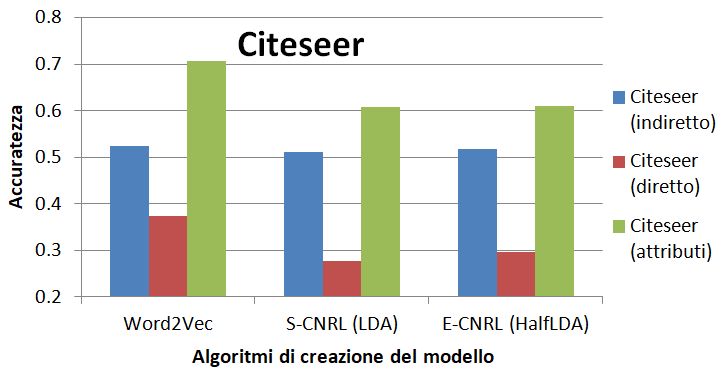
\includegraphics[width=\linewidth]{immagini/VC_citeseer}
	\caption{Andamento del grafo \citeseer, con 3 differenti algoritmi di creazione del modello e 3 diverse interpretazioni iniziali, valutato mediante l'accuratezza}
	\label{fig:VC_citeseer}
\end{figure}
%
Sull'asse delle ordinate vi sono i valori compresi nell'intervallo $[0, 1]$ misurati mediante la tecnica dell'accuratezza. Mentre sull'asse delle ascisse vi sono i tre algoritmi utilizzati per creare il modello del grafo partendo dai cammini. \wv è il metodo di controllo, mentre S-CNRL e E-CNRL che lavorano rispettivamente con LDA e HalfLDA, sono i nuovi algoritmi proposti. Entrambi per alcune parti continuano ad usare \wv.\\
Sia \cora che \citeseer sono grafi originariamente diretti (\textcolor{red}{misurazioni rosse}), tuttavia si è provato ad interpretarli anche come se fossero indiretti (\textcolor{blue}{campionamento blu}), l'ultimo andamento è dato dall'introduzione degli attributi (\textcolor{green}{dati verdi}).\\
Ecco alcuni dettagli che emergono dai due grafici:
\begin{itemize}
	\item \wv mostra prestazioni, anche se di poco, maggiori delle due alternative che invece tendono ad equivalersi
	\item la media dei valori delle misurazione nel grafico di \cora (Figura~\ref{fig:VC_cora}) è $0.696$ rispetto a quella di \citeseer (Figura~\ref{fig:VC_citeseer}) che è $0.491$, la prima risulta essere maggiore di circa $\displaystyle \frac{2}{10}$ questo è dovuto anche al fatto che \cora abbia una $\displaystyle densita' = \frac{archi}{nodi}$ maggiore rispetto a \citeseer
	\item un alta densità degli archi permette di creare molte interazioni fra i nodi e quindi il modello meglio rappresenta il grafo, si noti però che questo non è sempre facile da individuare, qui è presente uno stacco evidente in quanto entrambi i grafi hanno un estremamente bassa densità si dice infatti che sono sparsi
	\item si è provato ad aumentare la densità considerando ambo i grafi come indiretti (ogni arco indiretto può essere rappresentato come due archi diretti) si ha quindi poco meno di un raddoppio della densità, è infatti possibile che un arco avesse già il suo opposto e quindi non risente del cambiamento.
	L'effetto per entrambi è stato un innalzamento del valore medio lungo i 3 algoritmi usati
	\item con il grafo indiretto l'incremento di S-CNRL e E-CNRL è molto maggiore rispetto a quello di \wv questo può indicare, che \wv lavora molto bene con i grafi orientati a dispetto degli altri due metodi
	\item l'introduzione degli attributi tramite il grafo bipartito cambia notevolmente la situazione portando ad un incremento di prestazioni. Questi valori vanno confrontati con i dati del grafo orientato in quanto quello è il valore corretto, i punti blu del grafo non-orientato non sono comparabili in quanto servono a mostrare come la densità influisce sul risultato, rappresentano però un nuovo grafo diverso dall'originale, e quindi non paragonabile
\end{itemize}
%
\section{Valutazione dell'individuazione di comunità}
Questa sezione ripercorre il corpo principale del tirocinio, ossia l'integrazione degli attributi e la valutazione di un partizione mediante la modularità. Vengono presentate quattro situazioni ognuna approfondisce un aspetto affrontato.
%
\subsection{Confronto numero comunità}%1
%
\begin{figure}[htp]
	\centering
	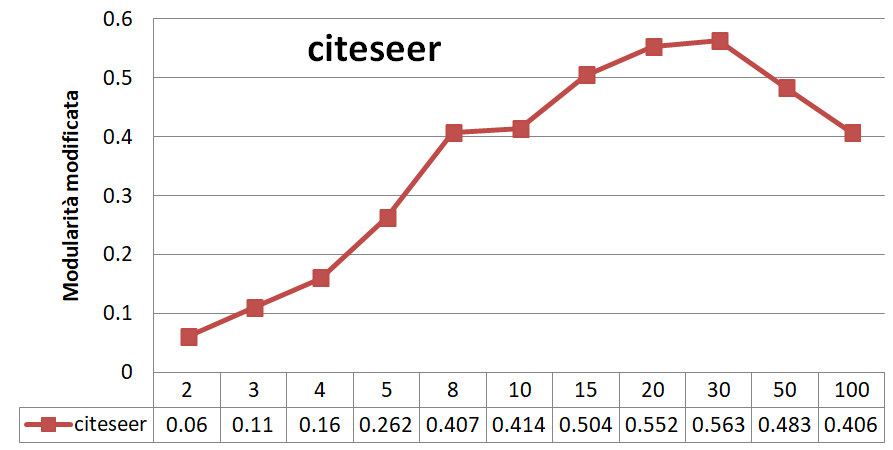
\includegraphics[width=\linewidth]{immagini/MOD_1_num_cmty}
	\caption{Accuratezza rappresentativa al variare del numero delle comunità da generare}
	\label{fig:MOD_1_num_cmty}
\end{figure}
%
In Figura~\ref{fig:MOD_1_num_cmty} è possibile vedere l'andamento dell'algoritmo di d'individuazione delle comunità LDA, applicato al grafo \citeseer di cui si considera solo la struttura, la valutazione vien fatta con la \mmod.\\
L'unico parametro che viene modificato è mostrato sull'asse delle ascisse ed è il numero di comunità che si vanno a ricercare all'interno del grafo. Ecco cosa s'osserva:
\begin{itemize}
	\item la progressione del numero di comunità da ricercare è stata scelta per mostrare la rapida crescita della modularità quando piccoli numeri sono coinvolti
	\item il valore calcolato su $2$ comunità è estremamente basso perché difficilmente riesce a rappresentare a dovere una vasta selezione di nodi
	\item la modularità cresce con l'aumentare delle comunità, che premiano sempre più le peculiarità del grafo
	\item c'è un massimo compreso fra $30$ e $50$ dove questa crescita s'interrompe
	\item gli ultimi due dati $50$ e $100$ decrescono, questo è noto come il \textbf{problema dell'overfitting}, a causa di un addestramento eccessivo il risultato raggiunto non è più in linea con le aspettative.\\
	Via via che i gruppi di nodi si stringono perdono di rappresentazione portando così ad un decremento della modularità. Si osserva questo fenomeno anche in Figura~\ref{fig:MOD_3_elaborazione}
\end{itemize}

\subsection{Metriche di valutazione}%2
Nella Tabella~\ref{tab:2_metriche} vengono mostrati i due grafi di \cora e \citeseer, valutati mediante tre differenti metriche di calcolo della modularità.\\
Ambo i grafi sono stati caricati senza considerare gli attributi dei nodi ma solo la loro struttura, la creazione del modello è avvenuta con S-CNRL e il suo algoritmo LDA, tramite cui sono state ricavate le $10$ comunità che vengono  valutate in Tabella.\\
\\
Non ha senso confrontare i tre differenti metodi di calcolo della modularità, in quanto premiano aspetti differenti. Inoltre ognuno si posiziona su un diverso ordine di grandezza, spicca sopratutto \mover che presenta tutti i valori molto vicini a 0, questo perché come riporta la Tabella~\ref{tab:dati_grafi} ambo i grafi sono estremamente sparsi e a causa di ciò \mover ha il valore assoluto della modularità calcolata vicino a $0$.\\
Tutti i metodi assegnano a \cora il valore più alto, e questo fa capire che se una partizione è nettamente migliore di un'altra allora verrà premiata indipendentemente dalla metrica di valutazione usata.\\
La \mmod è stata scelta come metrica ufficiale degli esperimenti, non solo per il fatto che è quella usata nell'articolo di \cnrl, ma anche perché presenta dei valori facilmente analizzabili e comprensibili, \mover funziona bene ma è sempre difficile comprendere i risultati a cui s'arriva rischiando incomprensioni.
%
\begin{center}
	% Schema num: 2 -> confronto metriche (cmty=10, no_att, valutazione con grafo norm, metric 8 -> HalfLDA)
	\begin{tabular}{|l|c|c|c|} % \multicolumn{2}{|c|}{testo}  \multirow{2}{*}{testo}   $ \e{-}$
		\hline
		\ & \mmax & \mover & \mmod \\
		\hline
		\cora & $2.04$ \e{-1} & $1.21$ \e{-5} & $5.31$ \e{-1} \\
		\citeseer & $8.42$ \e{-2} & $-3.55$ \e{-6} & $3.67$ \e{-1} \\
		%2.04E-01	1.21E-05	5.31E-01
		%8.42E-02	-3.55E-06	3.67E-01
		\hline
	\end{tabular}
	\captionof{table}{Confronto fra i metodi di modularità spiegati, partendo dal grafo normale con $10$ comunità}
	\label{tab:2_metriche}
\end{center}
%
\subsection{Confronto metodi d'elaborazione}%3
%
\begin{figure}[htp]
	\centering
	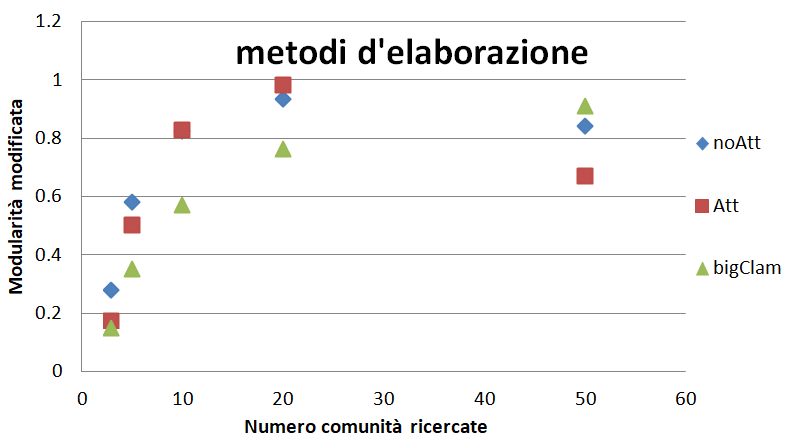
\includegraphics[width=\linewidth]{immagini/MOD_3_elaborazione}
	\caption{Prestazioni dei diversi procedimenti d'elaborazione del modello al variare del numero di comunità da ricercare (grafo \cora)}
	\label{fig:MOD_3_elaborazione}
\end{figure}
%
In Figura~\ref{fig:MOD_3_elaborazione} vengono confrontati tre differenti metodi d'elaborazione dei grafi, il cui scopo è trovare le comunità.\\
Viene presentato il grafo \cora su cui si è cercato d'individuare tramite una progressione da $3$ a $50$ comunità, tutte valutate in seguito tramite la \mmod. \\
I tre metodi utilizzati sono:
\begin{itemize}
	\item \textbf{noAtt}: si considera in partenza unicamente la struttura del grafo, dai cui si ricavano i cammini e vengono elaborati con LDA
	\item \textbf{Att}: oltre ai cammini derivanti dalla struttura si crea anche il grafo bipartito degli attributi, il tutto elaborato sempre mediante LDA
	\item \textbf{bigClam}: è il metodo tratto dall'articolo "Overlapping community detection at scale: a nonnegative matrix factorization approach"\cite{bigClam_paper}, implementato dall'università di Stanford\cite{bigClam_code}.\\
	È stato scelto come algoritmo di controllo per verificare l'andamento delle prestazioni di S-CNRL
\end{itemize}
Dalla Figura possiamo capire:
\begin{itemize}
	\item come avviene in Figura~\ref{fig:MOD_1_num_cmty} con l'aumentare del numero di comunità si ha il problema dell'overfitting, qui è lo stesso.\\
	Per \citeseer il problema si rivela quando si cercano $50$ comunità e analogo è per \cora, questo sembra non valere per bigClam anche se è inevitabile che accada con numeri molto alti di comunità cercate
	\item durante la crescita le prestazioni di bigClam restano costantemente inferiori
	\item l'apice è raggiunto mediante gli attributi con $20$ comunità ad un valore di $Q=0.986$, è importante notare non tutti gli apici dei vari metodi si posizionano a $20$ comunità, al contrario. BigClam sembra aver questo massimo oltre le $50$ comunità
	\item valutare il grafo mediante e senza gli attributi sembra non influire troppo, anche se così non dovrebbe essere (caso meglio analizzato in Tabella~\ref{tab:4_valutazioni})
\end{itemize}
%
\subsection{Confronto criteri di valutazione}%4
%
\begin{center}
	% Schema num: 4 -> confronto valutazioni
	\begin{tabular}{|cc|c|c|} % \multicolumn{2}{|c|}{testo}  \multirow{2}{*}{testo}   $ \e{-}$
		\hline
		\multicolumn{2}{|c|}{\textbf{\cora}} & \multicolumn{2}{|c|}{valutazione} \\
		\multicolumn{2}{|c|}{\ } & struttura & ipergrafo \\
		\hline
		\multirow{2}{*}{elaborazione} & noAtt & $8.24$ \e{-1} & $9.83$ \e{-3} \\
		& Att & $8.29$ \e{-1} & $2.33$ \e{-2} \\
		\hline
		\hline
		\hline
		\multicolumn{2}{|c|}{\textbf{\citeseer}} & \multicolumn{2}{|c|}{valutazione} \\
		\multicolumn{2}{|c|}{\ } & struttura & ipergrafo \\
		\hline
		\multirow{2}{*}{elaborazione} & noAtt & $4.14$ \e{-1} & $8.86$ \e{-6} \\
		& Att & $4.14$ \e{-1} & $2.30$ \e{-2} \\
		\hline
	\end{tabular}
	\captionof{table}{Misurazione delle comunità, generate attraverso due differenti metodi d'elaborazione, e analizzate su due tipologie di valutazione}
	\label{tab:4_valutazioni}
\end{center}
Nella Tabella~\ref{tab:4_valutazioni} vengono mostrati entrambi i grafi di \cora e \citeseer, su ognuno son state fatte quattro differenti valutazioni.\\
Sulle righe vi sono i metodi  d'elaborazione utilizzati per trovare le comunità:
\begin{itemize}
	\item \textbf{noAtt} indica che del grafo è stata utilizzata solamente la struttura per la generazione dei cammini
	\item \textbf{Att} indica invece che oltre ai dati della struttura vengono utilizzati anche gli attributi introdotti tramite un grafo bipartito
\end{itemize}
%
Sulle colonne sono invece riportati i due metodi per la valutazione della partizione generata:
\begin{itemize}
	\item \textbf{struttura} indica che il grafo utilizzato per la valutazione tramite \mmod è quello originale, che contiene appunto solo la struttura
	\item \textbf{ipergrafo} il grafo per la valutazione con \mmod contiene anche gli archi degli attributi, non è possibile utilizzare un grafo bipartito in quanto contiene nodi (l'insieme N2) non appartenenti al grafo originario, si opta quindi per l'ipergrafo.\\
	Quello qui utilizzato, rispetto a quello mostrato in Figura~\ref{fig:7transform_hyper}, mantiene anche gli archi originali e per non creare incoerenze considera tutti gli archi come diretti, ciò porta a più d'un raddoppio del numero d'archi, partendo da un numero base già elevatissimo
\end{itemize}
%
Dalla Figura~\ref{fig:MOD_3_elaborazione} si può vedere che con $10$ comunità la valutazione di \cora elaborato con e senza attributi è molto simile, s'è scelto d'utilizzare quindi le $10$ comunità per osservare le variazioni quando si adotta una valutazione attraverso l'ipergrafo.\\
Ecco cosa si può notare:
\begin{itemize}
	\item per la scelta del numero di comunità i dati di \cora valutati sulla struttura sono pressoché uguali
	\item per \citeseer accade o stesso, qui i due valori sono identici.\\
	Il dato di $4.14$ \e{-1} è già apparso in Tabella~\ref{fig:MOD_1_num_cmty}
	\item se la valutazione avviene sull'ipergrafo sia nel caso di \cora che di \citeseer il valore più alto viene generato con l'elaborazione effettuata sugli attributi.\\
	È in linea con le aspettative, perché i cammini aggiunti dal grafo bipartito vanno a descrivere una sezione che l'elaborazione utilizzante solo la struttura non può conoscere e quindi non vi si può adattare
	\item il fatto che tutte le valutazioni sull'ipergrafo sono così vicine allo $0$ è dovuto al fatto che l'Espressione~\ref{eq:d_in-out} parte della Formula~\ref{eq:m_mod} della \mmod in presenza di un grafo molto denso, ed è questo il caso, abbassa notevolmente il valore della misurazione
\end{itemize}
%
Nonostante i dati mostrati in Tabella~\ref{tab:4_valutazioni} siano perfettamente in linea con le aspettative, non è possibile affermare che quanto mostrato in questa sottosezione sia sempre vero in ogni possibile situazione, in quanto i risultati restituiti dalla \mmod presentano una non trascurabile variabilità.



\chapter{Conclusioni}
Cosa si scrive nelle conclusioni?

%\end{document}




					%capitolo 3
    %\input{4_lavori_futuri}					%capitolo 4
    %\input{5_conclusioni}					%capitolo 5
    \endgroup


    % bibliografia in formato bibtex
    % aggiunta del capitolo nell'indice
    \addcontentsline{toc}{chapter}{Bibliografia}
    % stile con ordinamento alfabetico in funzione degli autori
    \bibliographystyle{plain}
    %\bibliography{biblio}
%%%%%%%%%%%%%%%%%%%%%%%%%%%%%%%%%%%%%%%%%%%
%% Nota:
%%
%% Nella bibliografia devono essere riportati tutte le fonti consultate 
%% per lo svolgimento della tesi. La bibliografia deve essere redatta 
%% in ordine alfabetico sul cognome del primo autore. 
%% 
%% La forma della citazione bibliografica va inserita secondo la fonte utilizzata:
%% 
%% LIBRI
%% Cognome e iniziale del nome autore/autori, la data di edizione, titolo, casa editrice, eventuale numero dell’edizione. 
%% 
%% ARTICOLI DI RIVISTA
%% Cognome e iniziale del nome autore/autori, titolo articolo, titolo rivista, volume, numero, numero di pagine.
%% 
%% ARTICOLI DI CONFERENZA
%% Cognome e iniziale del nome autore/autori (anno), titolo articolo, titolo conferenza, luogo della conferenza (città e paese), date della conferenza, numero di pagine. 
%% 
%% SITOGRAFIA
%% La sitografia contiene un elenco di indirizzi Web consultati e disposti in ordine alfabetico. 
%% E’ necessario:
%%   Copiare la URL (l’indirizzo web) specifica della pagina consultata
%%   Se disponibile, indicare il cognome e nome dell’autore, il titolo ed eventuale sottotitolo del testo
%%   Se disponibile, inserire la data di ultima consultazione della risorsa (gg/mm/aaaa).    
%%%%%%%%%%%%%%%%%%%%%%%%%%%%%%%%%%%%%%%%%%%
%%%%%%%%%%%%%%%%%%%%%%%%%%%%%%%%%%%%%%%%%%%    

    \titleformat{\chapter}
        {\normalfont\Huge\bfseries}{Allegato \thechapter}{1em}{}
    % sezione Allegati - opzionale
    \appendix
    %\input{allegati}

\end{document}
